\documentclass[lettersize,journal]{IEEEtran}


\usepackage{setspace}

\usepackage{amsmath,amsfonts}
%\usepackage{algorithmic}
\usepackage{algorithm}
\usepackage{array}
\usepackage[caption=false,font=normalsize,labelfont=sf,textfont=sf]{subfig}
\usepackage{textcomp}
\usepackage{stfloats}
\usepackage{url}
\usepackage{verbatim}
\usepackage{graphicx}
\usepackage{cite}
\usepackage{bm}
\usepackage{pgfplots}

%
% extra


%  added
\usepackage{algorithm}
\usepackage{algpseudocode}
\usepackage{listings}
\usepackage{xcolor} %Optional: for customizing colors
\definecolor{mygreen}{rgb}{0,0.6,0}
\usepackage{array}  % for better column definitions
\usepackage{paralist}
\usepackage{colortbl}
\usepackage{amssymb}
\usepackage{pifont}

% Packages from Table_Thor.tex
\usepackage{amssymb}  % For \checkmark
\usepackage{tikz}
\usepackage{diagbox}  % For diagonal lines in table cells
\usepackage{adjustbox} % For adjusting position of the table
\usepackage{verbatim}
\usepackage{caption}
\usepackage{rotating}  % For rotating text
\usepackage{multirow}
\usepackage{makecell}  % For better cell formatting
\usepackage{arydshln}


% Title, Author, and other configurations
\title{\textsc{Thor}: A  Non-Speculative Value Dependent Timing Side Channel Attack Exploiting Intel AMX}
%A Novel Side-Channel Vulnerability in Intel AMX}
\author{Farshad Dizani, Azam Ghanbari, Joshua Kalyanapu, Darsh Asher, and Samira Mirbagher Ajorpaz}

% Setting the appearance of the code listing
\lstset{
    frame=single, % Adds a frame around the code
    language=C, % Syntax highlighting for C
    basicstyle=\ttfamily\small, % Sets the basic style
    breaklines=true, % Enables line breaking
    showstringspaces=false, % Don't show spaces in strings as special underscore characters
    tabsize=2, % Sets the tab size
    commentstyle=\color{mygreen}, % Comment color
    keywordstyle=\color{blue}, % Keyword color
    stringstyle=\color{red} % String literal color
}
% Defining a boxed style
\lstdefinestyle{boxed}{
    frame=single, % Adds a frame around the code
    xleftmargin=3pt,
    xrightmargin=3pt,
    aboveskip=4pt,
    belowskip=0pt,
}

% Defining a non-boxed style
\lstdefinestyle{nonboxed}{
    frame=none, % No frame around the code
    xleftmargin=0pt, % Adjust margins
    xrightmargin=0pt,
    aboveskip=4pt,
    belowskip=0pt,
}

\usepackage{graphicx}

% Custom commands from Table_Thor.tex
\newcommand{\fullcircle}{\tikz \fill (0,0) circle (0.8ex);}

\newcommand{\halfcircle}{%
  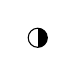
\begin{tikzpicture}
    \fill[black] (0,0) -- (0,0.8ex) arc[start angle=90,end angle=-90,radius=0.8ex] -- cycle;
    \fill[white] (0,0) -- (0,0.8ex) arc[start angle=90,end angle=270,radius=0.8ex] -- cycle;
    \draw (0,0) circle (0.8ex);
  \end{tikzpicture}%
}

\newcommand{\emptycircle}{\tikz \draw (0,0) circle (0.8ex);}

% Define commands for the squares
\newcommand{\darksquare}{%
    
\begin{tikzpicture}[scale=0.5]
        \fill[black] (0,0) rectangle (0.4,0.4);
    \end{tikzpicture}%
}

\newcommand{\lightsquare}{%
    
\begin{tikzpicture}[scale=0.5]
        \fill[gray] (0,0) rectangle (0.4,0.4);
    \end{tikzpicture}%
}

\newcommand{\halfsquare}{%
    
\begin{tikzpicture}[scale=0.5]
        \fill[gray] (0,0) rectangle (0.2,0.4);
        \fill[black] (0.2,0) rectangle (0.4,0.4);
    \end{tikzpicture}%
}

\newcolumntype{P}{>{\hspace{0.3cm}}p{0.9cm}}
\newcolumntype{C}{>{\centering\arraybackslash}m{3cm}}  % Category column
\newcolumntype{X}{>{\centering\arraybackslash}m{4cm}}  % Attack column


\hyphenation{op-tical net-works semi-conduc-tor IEEE-Xplore}

\newcommand{\paragrabf}[1]{\noindent \textbf{#1}\ }

\usepackage{titlesec}
\titlespacing{\section}{0pt}{*0.8}{*0.5}
\titlespacing{\subsection}{0pt}{*0.5}{*0.3} % Adjust spacing before and after % shorten the paper and then remove

%%%%%%From ISCA



%%%End of ISCA


\begin{document}

%\title{A Novel Side-Channel Vulnerability in Intel AMX}


% \thanks{Manuscript received November 4, 2023; revised February 28, 2024.}
% \thanks{The next few paragraphs should contain 
% the authors' current affiliations, including current address and e-mail. For 
% example, First A. Author is with the National Institute of Standards and 
% Technology, Boulder, CO 80305 USA (e-mail: author@boulder.nist.gov). }
% \thanks{Second B. Author and Third C. Author are with Rice University, Houston, TX 77005 USA. (e-mail: authorB@lamar.colostate.edu, authorC@abc.com).}
% }

% The paper headers
% \markboth{IEEE Journal of \LaTeX\ Class,~Vol.~12, No.~6, February~2024}%
% {Shell \MakeLowercase{\textit{et al.}}: A Sample Article Using IEEEtran.cls for IEEE Journals}

% \IEEEpubid{0000-0000~\copyright~2024 IEEE}
% Remember, if you use this you must call \IEEEpubidadjcol in the second
% column for its text to clear the IEEEpubid mark.

 \maketitle

 % \section{Introduction}



\begin{spacing}{0.96}
    
\begin{abstract}  
Test time scaling is currently one of the most active research areas that shows promise after training time scaling has reached its limits.
Deep-thinking (DT) models are a class of recurrent models that can perform easy-to-hard generalization by assigning more compute to harder test samples.
However, due to their inability to determine the complexity of a test sample, DT models have to use a large amount of computation for both easy and hard test samples.
Excessive test time computation is wasteful and can cause the ``overthinking'' problem where more test time computation leads to worse results.
In this paper, we introduce a test time training method for determining the optimal amount of computation needed for each sample during test time.
We also propose Conv-LiGRU, a novel recurrent architecture for efficient and robust visual reasoning. 
Extensive experiments demonstrate that Conv-LiGRU is more stable than DT, effectively mitigates the ``overthinking'' phenomenon, and achieves superior accuracy.
\end{abstract}  

\begin{IEEEkeywords}
Intel Advanced Matrix Extensions (AMX), Value-dependent timing side-channel, ML privacy, NN sparsity.
\end{IEEEkeywords}

\section{Introduction}
%\IEEEPARstart{P} 
Privacy of machine learning models deployed on Machine Learning as a Service (MLaaS) platforms can be compromised by 
%have been facing growing scrutiny due to significant vulnerabilities that attackers can exploit to compromise critical aspects of these systems. These vulnerabilities allow 
adversaries to extract sensitive details, including model architecture
and hyperparameters~\cite{TramerZJRR16}. 
%, which are often proprietary and essential to the performance and commercial value of the model.
%These attacks are often based on gradient based inference, path-searching and surrogate model training methods to leak the target data. Adversary can train shadow models based on the output of the target model and then based on the confidence score leak the members on which model is trained.
%Trusted Execution Environments (TEEs) offer a secure enclave within a processor, safeguarding sensitive data and code from unauthorized access, even if the operating system is compromised. They protect against threats such as malicious software and physical attacks such as memory bus snooping. The CPU acts as the root of trust, establishing secure enclaves with hardware-enforced encryption and attestation. Intel SGX is a prime example, creating isolated "enclaves". TEEs like SGX are increasingly used to secure ML models (e.g., Slalom \cite{tramèr2019slalomfastverifiableprivate}, DarkneTZ \cite{Mo2020DarkneTZ}, TEESlice \cite{li2024teesliceprotectingsensitiveneural}, Occlumency \cite{Lee2019Occlumency}). These works leverage TEEs to protect sensitive computations and data within isolated enclaves, mitigating model stealing and unauthorized access risks. Being more efficient than cryptographic techniques, TEEs are being utilized as the root of trust by most current MLaaS applications to secure ML models.
% \begin{comment}
% *** Commenting Original Text***
% However, we show that as hardware accelerators become more deeply embedded %\cite{jeong2021rasa,jeong2023vegeta,nassif2022sapphire 
% \cite{intel2023amx}, they bring unique challenges for AI security that existing research has yet to explore fully. We show that the tight integration of on-core AI accelerators like Intel AMX  introduces a timing side channel that bypasses conventional defenses like speculative execution mitigations %~\cite{yan2018invisispec}
% or cache isolation %~\cite{kiriansky2018dawg}
% .
% \end{comment}
However, this paper shows that 
%as hardware accelerators become more deeply embedded %\cite{jeong2021rasa,jeong2023vegeta,nassif2022sapphire 
%\cite{intel2023amx}, they bring unique challenges for AI security that existing research has yet to explore fully. We show that
the tight integration of on-core AI accelerators like Intel AMX\cite{intel2023amx} causes AMX performance to depend upon operand value which works as proxy, enabling timer attacks on ML models thus introducing a timing side channel that bypasses conventional defenses like speculative execution mitigations %~\cite{yan2018invisispec}
or cache isolation %~\cite{kiriansky2018dawg}
and challenges the architectural and data privacy of ML.

\begin{comment}

Intel AMX's versatility supports both training and inference workloads in AI applications. Bfloat16 operations balance precision and dynamic range, making them suitable for neural network training, %~\cite{googleBFloat16Secret} 
while 8-bit integer operations enhance inference performance with negligible accuracy loss, providing significant acceleration for modern AI workloads. 
    
\end{comment}

\begin{comment}
*** Commenting Original Text***
We show that AMX performance depends on an operand value.
%as shown in Figure~\ref{fig:Cumulative_execution_time}.   
This dependency works as a proxy that
extends beyond traditional side channels, enabling timer attacks on machine learning models that challenge the architectural and data privacy of ML. 

\end{comment}



%\subsection{Microarchitectural Side Channel Attacks}
%\textbf{Transmission Channels.} 
Cache attacks exploit timing variations between accessing or flushing data in cache levels or DRAM~\cite{GrussFlushFlush}.
%.Prime+Probe%~\cite{prime_probe}
%, Flush+Reload%~\cite{flush+reload}
%, and Flush+Flush
 %\textcolor{red}{1 cite? }rely on cache set monitoring or eviction timing.
Spectre~\cite{kocher2020spectre} and Meltdown~\cite{meltdown} exploit speculative execution and exception handling. 
%Variants like Foreshadow %~\cite{van2018foreshadow} and LVI %~\cite{lvi} breach SGX and inject malicious data. %RIDL%~\cite{ridl}, Fallout%~\cite{canella2019fallout}, and Zombieload%~\cite{schwarz2019zombieload}
MDS Attacks~\cite{schwarz2019zombieload,canella2019fallout} target microarchitectural buffers. Defenses include cache partitioning~\cite{kiriansky18dawg}, 
%~\cite{herdrich2016cache,kiriansky18dawg}
Invisispec~\cite{yan2018invisispec}, privileged access controls (e.g., RAPL restrictions)~\cite{Lipp2021Platypus}, SMT disabling and other patches with performance overhead. 
%, and TurboBoost mitigation. 
%~\cite{wang2022hertzbleed}. 
%
However, no work has been done on the security evaluation of newly built Intel AMX for AI applications.


% \noindent\textbf{Speculative and Transient-Execution Attacks.}  %NetSpectre~\cite{schwarz2019netspectre} demonstrates remote speculative attacks using AVX timing.



%\subsection{Attacks on ML}
%\noindent\textbf{Model and Hyperparameter Extraction.} 
Black-box attacks extract model functionality or hyperparameters with minimal access but require confidence scores and are mitigated by  various methods like limiting the query rate, obfuscating the input data by masking, rounding confidence, or using homomorphic encryption.  
%Model inversion attacks~\cite{Fredrikson2015ModelInversion,Wand2022VarModelInversion} reconstruct sensitive inputs such as facial images.
%\noindent\textbf{Physical and Microarchitectural Attacks on ML.} 
Early physical attacks, such as IKWYS~\cite{wei2018know}  %and CSI NN~\cite{CSINN2018}, 
used power or EM side channels to infer neural network (NN) parameters but required physical access. %. Cache Telepathy
~\cite{Yan2020Cachetelepathy} 
%and DeepRecon~\cite{HongDeepRecon2018} 
leverages cache timing to leak NN architecture but is reliant on particular ML libraries and co-location. 
%Rowhammer-based attacks like DeepSteal~\cite{RakinDeepSteal2021} leak partial weights but assume partial black-box knowledge~\textcolor{red}
 We confirmed that vulnerabilities on NNs using floating-point timing~\cite{9218707} have been completely mitigated in the Intel AMX design and thus are no longer available to the attacker. 
%Despite advances, non-cache based microarchitectural side-channel attacks targeting NN parameters remain unexplored.

%  Traditionally, power side-channel attacks require physical access to a system to measure power consumption or electromagnetic emissions. Such attacks are less common and practical because they require a high level of access. However, Lipp et al. \cite{Lipp2021Platypus} demonstrated a method to exploit the Running Average Power Limit (RAPL) interface for power side-channel attacks without needing physical access. However, RAPL is now a privileged interface, making this technique inaccessible to the unprivileged attacker. 
% %
% Dynamic Voltage and Frequency Scaling (DVFS), an optimization technique for power management, can paradoxically open up new attack surfaces by converting power side channels into timing attacks. This vulnerability was exploited in Hertzbleed \cite{wang2022hertzbleed} to leak data by throttling under power limits, and in Collide+Power \cite{kogler2023collide+}, where power limits and throttling were manipulated to convert the memory power side channels into timing variations. Notably, power limit controls are usually privileged, and throttling can be mitigated by disabling Turbo Boost. As such, our work reveals a new, generic vulnerability in Intel AMX, specifically within its power and performance management mechanisms. Interestingly, unlike DVFS-related vulnerabilities, our discovered vulnerability persists irrespective of DVFS states and allows for exploitation regardless of whether DVFS is on or off. Additionally, our attack does not require a shared cache—unlike Collide+Power, which necessitates shared cache access to leak data, is now patched and leaks significantly lower rate (4.82 compared to 76.8 bits per hour for our attack).

 In this paper, we demonstrate the feasibility of exploiting Intel AMX 
 %this newly discovered vulnerability in NN operations 
 to leak sensitive information in NN, such as sparsity of it's weights. Inferring sparsity could inadvertently reveal sensitive data patterns. Understanding the sparsity pattern might provide insights into the underlying data distributions, potentially breaching data privacy.
Additionally, knowledge of sparsity patterns could enable attackers to craft more effective adversarial attacks. By understanding the structure of a model, an attacker might design inputs that strategically exploit sparsity, leading to degraded model performance or incorrect predictions.
 %Previous works in the literature have targeted NN models to infer architectural details, inputs, and weights, often necessitating physical access for power and electromagnetic measurements \cite{CSINN2018} or shared cache manipulation via known cache side channels \cite{Yan2020Cachetelepathy}.  
 Our approach is notable for not requiring physical access or a shared cache, unlike previous works %in the literature have targeted NN models to infer architectural details, inputs, and weights, 
 that often necessitating physical access for power and electromagnetic measurements 
 %\cite{CSINN2018} 
 or shared cache manipulation via known cache side channels \cite{Yan2020Cachetelepathy}, lowering the bar for potential attackers.
%Specifically, we investigate the behavior of AMX multiplication.
%, which operates in five distinct states and fluctuates between 52 and 20,000 cycles. 
We discover that the execution times of the Intel AMX multiplications vary depending on the operand's value. 
%are not consistent when AMX is transitioning between different states. 
%However, t
\begin{comment}
This phenomenon is different from the observed Hertzbleed~\cite{wang2022hertzbleed} because our attack continues to function even with the Intel Turbo Boost (DVFS) feature turned off, suggesting a novel root cause specific to the Intel AMX design compared to the Hertzbleed that relies on DVFS feature enabled and obsolete cryptographic libraries. 
\end{comment}
% New
This phenomenon is different from the observed Hertzbleed\cite{wang2022hertzbleed, liu2022frequency}, which is a side-channel attack that leverages dynamic voltage and frequency scaling (DVFS) on modern x86 processors to transform power fluctuations into timing attacks, extractable without direct power measurement. Hertzbleed exploits CPU frequency variations, linked to data-dependent power consumption. Our attack continues to function even with the Intel Turbo Boost (DVFS) feature turned off, suggesting a novel root cause specific to the Intel AMX design compared to Hertzbleed, which relies on the DVFS feature being enabled and obsolete cryptographic libraries.
Our attack also bypasses TEE based defenses in contrary to Rowhammer-based attacks like DeepSteal~\cite{RakinDeepSteal2021} that leak partial weights but can be protected by TEE-based defenses. 
%assume partial black-box knowledge

%Particularly, after exiting high-latency states and before stabilizing to a steady state, the execution time becomes a data-dependent process. 
%This dependency arises because 

%Our reverse engineering suggests that Intel AMX has a separate clock from the CPU clock and skipping the zero values in the multiplication operands of the accelerator influence the trend of frequency adjustments by leading to less power consumption, creating exploitable and unique timing differences.
%
%We demonstrate the exploitation of this side-channel vulnerability, showing that the execution time of AMX multiplications can be systematically measured to infer the sparsity of hidden weights of a NN. In this first study,
%our practical example, 
We successfully leaked zeros in 64 hidden weights with 100\% accuracy within 50 minutes of observation without access to the NN output value, confidence score or shared cache bypassing state of the art defenses such as obfuscation, masking or rounding confidence values of NN and cache defenses.
% 
Our proof of concept (PoC) attack  (\textsc{Thor}) represents the first step toward a new direction in ML privacy attacks. It is an attack on a single-layer NN but its significance is that, unlike prior approaches that rely on {{confidence scores}}, logits,  physical access, or higher privilege, \textsc{Thor} leverages timing information alone to infer critical and private parameters like NN's weight sparsity patterns and distributions. 
%Thor is fast but is limited to a single layer NN.

This paper presents the following contributions:
\begin{compactitem}
\item It characterized and reverse-engineered the Intel AMX, 
% data-dependent timing 
uncovering 
%its unique exploitable properties of Intel AMX features
%\item It identifies 
a novel type of data-dependent timing side-channel vulnerability within the Intel AMX accelerator.

\item It demonstrates the techniques necessary to exploit this newly discovered timing side-channel for launching attacks on NNs. Specifically, it illustrates how to determine the sparsity of NN weights by measuring execution time.
We show that the \textsc{Thor} leakage rate is 631\% and 1,493\% higher than the maximum leakage rates in the Hertzbleed and Collide+Power~\cite{kogler2023collide+} attacks, respectively.
\item We discuss defenses, propose a counter-measurement and measure its overhead on power consumption (2.59\% to 12.33\%).   
\end{compactitem}
\vspace{0.1em}
\textbf{Responsible disclosure.}  We reported our attack and findings to Intel in May 2024 and Intel confirmed our findings. %Moreover, we are planning to open source our code.




% \section{Background \& Related Works}
% \subsection{}
% The discoveries of Spectre \cite{kocher2019spectre} and Meltdown \cite{meltdown} showed how speculative execution and architectural optimizations could be exploited in the form of side  channels exposing private data through the foundations of optimization and subtle timing differences. Subsequent research 
% uncovered an avalanche of vulnerabilities targeting various micro-architectural components such as 
% %on other atta~\cite{pandorasbox} 
% caches ~\cite{prime_probe, flush+reload, GrussFlushFlush, osvik2006cache}, internal CPU buffers ~\cite{kocher2019spectre,Phantom2023,spectre_here_to_stay2019, SpectreV4,kiriansky2018speculative,koruyeh2018spectre,maisuradze2018ret2spec,meltdown, canella2018systematic,van2018foreshadow,lvi, moghimi2020medusa,ridl,
% schwarz2019zombieload, canella2019fallout, moghimi2023downfall}, prefetcher ~\cite{gruss2016prefetch,lipp2022amd,augury,gofetch2024}, PACMAN~\cite{PACMAN}, TLB ~\cite{Tatar2022tlbdr,gras_translation_2018,koschel2020tagbleed}, port contention~\cite{bhattacharyya2019smotherspectre}, scheduler queues~\cite{SQUIP2023}, micro-op cache~\cite{uop2021Ashish}, exploiting other shared micro-architectural components~\cite{CrossTalk2021, weber2021osiris} and remote attacks~\cite{Brumley2003Remote,Bernstein2005,Aciicmez2007d,Crosby2009,Beery2013TIME,VanHoef2016Heist,VanGoethem2020Timeless,Irazoqui2015Lucky,schwarz2019netspectre,schwarzl2023practical, Schwarzl2022Remote,Gruss2019page,Kurt2020Netcat, wang2022hertzbleed,Zhao2009cache},   fundamentally reshaped our understanding of processor security. 

% However, no work has been done on security evaluation of Intel AMX.  

% \subsection{Intel AMX Architecture and Instructions.}
% Intel AMX is an integrated accelerator introduced with the 4th Gen Intel Xeon Scalable processors, specifically engineered to boost the efficiency of matrix computations. %Figure~\ref{fig:AMX-arch} illustrates the Intel AMX architecture.

% AMX introduces a new set of registers and instructions. The registers in Intel AMX are known as Tiles, a new concept in Intel CPUs that provide a matrix of data registers, as opposed to the traditional vector registers seen in previous SIMD architectures like AVX-512. AMX includes 8 Tile registers, each capable of holding up to 16 rows with 64 bytes per row, amounting to a total of 1 KB per Tile. The number of rows and the number of bytes per row can be adjusted using the LDTILECFG instruction, and this configuration information is stored as metadata in a control register known as TILECFG. Once this configuration is set, AMX instructions such as load, store, and matrix multiplication will operate according to the specified dimensions for each Tile. Intel AMX instructions are synchronized with the Intel Architecture host (IA host) instruction stream, and the Tile loads and stores are coherent with the host memory \cite{Intel_Arc_Ins_Set_Extensions}.

% Tile Matrix Multiply unit (TMUL) serves as the accelerator engine for executing multiplication calculations. When using full-size Tile operands, the latency of the multiplication instruction is 52 cycles, while pipelining allows for a throughput of 16 cycles. Intel AMX supports two data types: BF16 and INT8. Consequently, it can perform 512 multiplications and 512 additions per cycle for BF16 and 1024 multiplications and 1024 additions per cycle for INT8 \cite{IntelOptRefManual}. 

\begin{comment}
AMX instructions utilize port 5 as their dedicated execution port. When two hyper-threads are active within a core, they compete for the same resources to execute AMX instructions.
\end{comment}

% \subsection{Microarchitectural Side Channel Attacks}
% %\textbf{Transmission Channels.} 
% Cache attacks exploit timing variations between cache levels or DRAM. Prime+Probe%~\cite{prime_probe,osvik2006cache}
% , Flush+Reload%~\cite{flush+reload}
% , and Flush+Flush~\cite{GrussFlushFlush} rely on cache set monitoring or eviction timing.  Spectre~\cite{kocher2020spectre} and Meltdown~\cite{meltdown} exploit speculative execution and exception handling. Variants like Foreshadow %~\cite{van2018foreshadow} 
% and LVI %~\cite{lvi} 
% breach SGX and inject malicious data. RIDL %~\cite{ridl}
% , Fallout%~\cite{canella2019fallout}
% , and Zombieload %~\cite{schwarz2019zombieload} 
% target microarchitectural buffers. Defenses include cache partitioning
% %~\cite{herdrich2016cache,kiriansky18dawg}
% , Invisispec
% %~\cite{Invisispec}
% , privileged access controls (e.g., RAPL restrictions), SMT disabling, and TurboBoost mitigation. 
% %~\cite{wang2022hertzbleed}. 

% However, no work has been done on security evaluation of Intel AMX.


% % \noindent\textbf{Speculative and Transient-Execution Attacks.}  %NetSpectre~\cite{schwarz2019netspectre} demonstrates remote speculative attacks using AVX timing.



% \subsection{Attacks on ML}
% %\noindent\textbf{Model and Hyperparameter Extraction.} 
% Black-box attacks extract model functionality~\cite{TramerZJRR16,Orekondy18Knock} or hyperparameters~\cite{wang2018hyperparameters} with minimal access but require confidence scores and are mitigated by  various methods \textcolor{red}{TODO}. 
% %Model inversion attacks~\cite{Fredrikson2015ModelInversion,Wand2022VarModelInversion} reconstruct sensitive inputs such as facial images.
% %\noindent\textbf{Physical and Microarchitectural Attacks on ML.} 
% Early physical attacks, such as IKWYS~\cite{wei2018know} and CSI NN~\cite{CSINN2018}, used power and EM side-channels to infer neural network (NN) parameters but require physical access. Cache Telepathy~\cite{Yan2020Cachetelepathy} and DeepRecon~\cite{HongDeepRecon2018} leverage cache timing to leak NN architecture but are reliant on particular ML libraries and co-location. Rowhammer-based attacks like DeepSteal~\cite{RakinDeepSteal2021} leak partial weights but assume partial black-box knowledge.
%  We confirmed that attacks on neural networks using floating-point timing vulnerabilities~\cite{9218707} have been largely mitigated by modern accelerators such as Intel AMX. %Recent attacks like DeepRecon~\cite{HongDeepRecon2018} focus on architecture and parameter extraction but fail to address MIA comprehensively.

% Despite advances, direct microarchitectural side-channel attacks targeting neural network parameters remain unexplored.

\section{Threat Model}
The attacker and victim are two distinct processes running on the same server. These processes are entirely isolated in terms of address space and can be executed on different CPU cores. As shown in Figure \ref{fig:Thor-threat-model}, the victim process is an API that runs a NN designed for specific tasks and utilizes Intel AMX for matrix computations. The attacker process, which operates as a non-privileged user, does not have direct access to the model’s parameters but interacts with the model via the inference API. The attacker sends crafted inputs to the inference API and measures the timing of the victim process's responses. By examining timing variations, the attacker can gain insights into the NN's internal parameters by taking advantage of the timing differences caused by Intel AMX computations. We assume cache defenses are deployed or there is no shared cache,  thus channels such as \cite{Yan2020Cachetelepathy} is not available to the adversary. The ML model is a single layer NN protected by obfuscated the confidence score and the output by methods such as adding noise or rounding confidence scores \cite{Fredrikson2015ModelInversion}. The victim may leverage TEEs, Intel SGX, to execute the NN computations within isolated enclaves.


% \textsc{Thor} exploits Intel AMX timing variations to infer sparsity patterns in neural network weights hosted on inference APIs. As a non-privileged attacker, it sends tailored inputs and measures response times, leveraging amplified timing differences in AMX Warm-State transitions to detect zero weights.
% % The attack works for both binary and non-binary weight patterns without requiring confidence scores, logits, or training data. It is adaptable to diverse environments, including cloud systems, MLaaS platforms, and SGX enclaves. By avoiding reliance on shared memory or privileged interfaces (for example, Flush + Reload, PlatyPus), and speculative or physical access attacks (for example, Specter, EM based methods), \textsc{Thor} offers a purely timing-based approach. Thor is limited to a single-layer neural network.

\begin{figure}[!ht] %\vspace{-5mm}
    \centering
   \includegraphics[width=\linewidth]{images/threat_model_v4.pdf} 
    \caption{\textsc{Thor} Threat Model.}
    \label{fig:Thor-threat-model}
\end{figure}


% %{System Configuration.} 
% Our investigations utilized a server running {Red Hat Enterprise Linux release 9.4} with {Linux kernel version 5.14}, powered by an { Intel Xeon Gold 5420+} from the {Sapphire Rapids microarchitecture}. 
% %
% The tests were carried out with a range of configurations,
% %shown in Table~\ref{tab:configurations}, 
% including the { autonomous (hardware-only)} and { cooperative P-state control modes}, under {minimal power}, {maximum performance}, and {efficiency-focused} platform power settings. {Turbo Boost} was tested in both {enabled} and {disabled states}. {Prefetchers} were toggled between {enabled} and {disabled states} across experiments to assess their impact on noise and timing variations. The server configurations included the UEFI firmware versions SRV650-v3-3.14 (May 2024) and SRV650-v3-3.20 (June 2024), with the latter mitigating certain Spectre variants but remaining vulnerable to our attack, \textsc{Thor}.

\vspace{-1em}\section{Thor}
%{System Configuration.} 
Our investigations utilized a server running {Red Hat Enterprise Linux release 9.4} with {Linux kernel version 5.14}, powered by an { Intel Xeon Gold 5420+} from the {Sapphire Rapids microarchitecture}. 
%
The tests were carried out with a range of configurations,
%shown in Table~\ref{tab:configurations}, 
including the { autonomous (hardware-only)} and { cooperative P-state control modes}, under {minimal power}, {maximum performance}, and {efficiency-focused} platform power settings. {Turbo Boost} was tested in both {enabled} and {disabled states}. {Prefetchers} were toggled between {enabled} and {disabled states} across experiments to assess their impact on noise and timing variations. The server configurations included the UEFI firmware versions SRV650-v3-3.14 (May 2024) and SRV650-v3-3.20 (June 2024), with the latter mitigating certain Spectre variants but all above settings remains vulnerable to our attack. 
%, \textsc{Thor}.

%\subsection{Intel AMX Architecture and Instructions.}
\subsection{Reverse Engineering}
Intel AMX is an on-core accelerator introduced with the 4th Gen Intel Xeon Scalable processors, specifically engineered to boost matrix computation efficiency.
%Figure~\ref{fig:AMX-arch} illustrates the Intel AMX architecture.
%
%AMX introduces a new set of registers and instructions. The registers in Intel AMX are known as Tiles, a new concept in Intel CPUs that provides a matrix of data registers, as opposed to the traditional vector registers seen in previous SIMD architectures like AVX-512. AMX includes eight Tile registers, each capable of holding up to 16 rows with 64 bytes per row, amounting to 1 KB per Tile. 
%The number of rows and the number of bytes per row can be adjusted using the LDTILECFG instruction, and this configuration information is stored as metadata in a control register known as TILECFG. Once this configuration is set, AMX instructions such as load, store, and matrix multiplication will operate according to the specified dimensions for each Tile. Intel AMX instructions are synchronized with the Intel Architecture host (IA host) instruction stream, and the Tile loads and stores are coherent with the host memory \cite{Intel_Arc_Ins_Set_Extensions}.
Tile Matrix Multiply unit (TMUL) is the accelerator engine for executing multiplication calculations. 
%When using full-size Tile operands, the latency of the multiplication instruction is 52 cycles, while pipelining allows for a throughput of 16 cycles. 
%Intel AMX supports two data types: BF16 and INT8. Consequently, it  Intel AMX can perform 512 multiplications and 512 additions per cycle for BF16 and 1024 multiplications and 1024 additions per cycle for INT8 \cite{IntelOptRefManual}. 
Intel AMX can perform 512 and 1024 multiplications/additions per cycle for BF16 and INT8, respectively~\cite{IntelOptRefManual}. 
% \subsection{Dynamic Power/Performance Vulnerabilities of Intel AMX}
%In this section we explore AMX features that have the potential to be exploited in a transmission channel part of a microarchitectural attack.x

%








% \begin{tcolorbox}[ colback=lightgray!20,
% colframe=gray!50,
% boxrule=0.3mm,
% arc=2mm,
% width=0.48\textwidth,
% sharp corners=all, left=2mm,
% right=2mm,
% top=1mm,
% bottom=1mm
% ] These findings demonstrate that Intel AMX includes a frequency management unit that controls the operating frequency of the TMUL accelerator. This unit can potentially access or create frequencies that differ from the CPU frequency as shown as Transition Behavior of AMX Frequency to CPU Frequency in Warm State. 
% This finding is in contrast to the root cause known for AVX performance variation, known as power up/down~\cite{netspectre} which does not vary to match  the core frequency.  
% \end{tcolorbox}

%\begin{figure}[!hbp]
%\centering\includegraphics[width=0.4\textwidth]{images/Freq_transition.pdf}
%\caption{Illustration of AMX Frequency Adjustment During Transition Periods: (a) shows the transition to a 1.2 GHz CPU frequency, with intermediate operation at 1 GHz; (b) demonstrates the adjustment to a 2 GHz CPU frequency, passing through 1 GHz and 1.3 GHz stages.}
%\label{fig:Freq_transition}
%\end{figure}
%{\color{blue} Put Freq\_transition figure here}



% \begin{figure}[ht!]
%     \centering
%     \begin{tikzpicture}
%         \begin{axis}[
%             font=\scriptsize,
%             width=\linewidth*0.7,
%             height=\linewidth*0.32,
%             bar width=50,
%             xmin=21800, xmax=24650,
%             ybar,
%             ylabel={Frequency},
%             ylabel style={yshift=0pt},
%             ymin=0, ymax=0.006,
%             legend style={
%                 legend columns=1, 
%                 at={(1.01,0.5)}, 
%                 anchor=west,   
%                 font=\tiny,
%             },
%             legend image code/.code={\draw[fill=#1,draw=none] (0cm,-0.1cm) rectangle (0.25cm,0.1cm);},
%             legend entries={100\% sparsity, 50\% sparsity, 0\% sparsity}
%         ]
%             \addplot+[hist={density, bins=50}, fill=lightgray, draw=none] table[y index=0] {Diagrams/Data/100-0.txt};
%             \addplot+[hist={density, bins=50}, fill=black, draw=none] table[y index=0] {Diagrams/Data/100-half.txt};
%             \addplot+[hist={density, bins=50}, fill=gray, draw=none] table[y index=0] {Diagrams/Data/100-1.txt};
%         \end{axis}
%         \node[anchor=south east] at (rel axis cs:-0.05,1) {(a)};
%     \end{tikzpicture}
%     \begin{tikzpicture}
%         \begin{axis}[
%             font=\scriptsize,
%             width=\linewidth*0.7,
%             height=\linewidth*0.32,
%             bar width=50,
%             xmin=35500, xmax=56000,
%             ybar,
%             ylabel={Frequency},
%             ylabel style={yshift=0pt},
%             ymin=0, ymax=0.00205,
%             legend style={
%                 legend columns=1, 
%                 at={(1.01,0.5)}, 
%                 anchor=west,   
%                 font=\tiny,
%             },
%             legend image code/.code={\draw[fill=#1,draw=none] (0cm,-0.1cm) rectangle (0.25cm,0.1cm);},
%             legend entries={100\% sparsity, 50\% sparsity, 0\% sparsity}
%         ]
%             \addplot+[hist={density, bins=60}, fill=lightgray, draw=none] table[y index=0] {Diagrams/Data/1000-0.txt};
%             \addplot+[hist={density, bins=60}, fill=black, draw=none] table[y index=0] {Diagrams/Data/1000-half.txt};
%             \addplot+[hist={density, bins=60}, fill=gray, draw=none] table[y index=0] {Diagrams/Data/1000-1.txt};
%         \end{axis}
%         \node[anchor=south east] at (rel axis cs:-0.05,1) {(b)};
%     \end{tikzpicture}
%     \begin{tikzpicture}
%         \begin{axis}[
%             font=\scriptsize,
%             width=\linewidth*0.7,
%             height=\linewidth*0.32,
%             bar width=50,
%             xmin=170000, xmax=345000,
%             xlabel={Execution time (cycle)},
%             ybar,
%             ylabel={Frequency},
%             ylabel style={yshift=0pt},
%             ymin=0, ymax=0.00022,
%             legend style={
%                 legend columns=1, 
%                 at={(1.01,0.5)}, 
%                 anchor=west,   
%                 font=\tiny,
%             },
%             legend image code/.code={\draw[fill=#1,draw=none] (0cm,-0.1cm) rectangle (0.25cm,0.1cm);},
%             legend entries={100\% sparsity, 50\% sparsity, 0\% sparsity}
%         ]
%             \addplot+[hist={density, bins=60}, fill=lightgray, draw=none] table[y index=0] {Diagrams/Data/10000-0.txt};
%             \addplot+[hist={density, bins=60}, fill=black, draw=none] table[y index=0] {Diagrams/Data/10000-half.txt};
%             \addplot+[hist={density, bins=60}, fill=gray, draw=none] table[y index=0] {Diagrams/Data/10000-1.txt};
%         \end{axis}
%         \node[anchor=south east] at (rel axis cs:-0.05,1) {(c)};
%     \end{tikzpicture}
% \caption{Data Dependent AI computation: Cumulative Execution Time of Programs with varying zero bits in the TMUL operand of Intel AMX.}
% \label{fig:Cumulative_execution_time}
% \end{figure}

%\subsection{Non-speculative Value-based Vulnerability}

%\subsubsection{Value Dependency of Transition Time} \label{sec:valuedependencyofTransitionTime}
We studied the impact of operand sparsity on TMUL operations. % in Warm State.
%In our investigation of the TMUL execution time transition in the Warm State, we discovered an interesting effect involving zero values in the Tile operands during multiplication. 
By varying the number of zero values in the Tile operands during multiplication, we observed that increasing the number of zeros accelerates the 
AMX execution. 
%transition period. 
This effect is illustrated in Figure~\ref{fig:Cumulative_execution_time}
%\ref{fig:Effect_of_zeros_on_transition}
, which presents three distinct distributions showing the sparsity levels of the operand: 100\% sparsity, 50\% sparsity, and 0\% sparsity. 
The results indicate that a greater sparsity of operands in the tile operands leads to faster 
execution of the TMUL. The program with 1,000 AMX multiplications averages 54,005 cycles when operands have 0\% sparsity. Increasing sparsity to 50\% and 100\% reduces the average execution time to 45,953 and 38,747 cycles, respectively. In this case, 50\% and 100\% more sparsity make the execution 17.5\% and 39.4\% faster, respectively.
%Consequently, the execution time of a program that utilizes AMX multiplications is closely associated with the sparsity of its input operands. In Figure \ref{fig:Cumulative_execution_time}, we demonstrate this relationship 
%by executing 
%three test programs with 100, 1000, and 10,000 AMX multiplications, each 
%with varying levels of tile operand sparsity (0\%, 50\%, and 100\%). Each scenario was executed 1,000 times to construct the histogram. Our results reveal that varying sparsity levels significantly impact the execution time of AMX multiplications, with increased sparsity leading to faster program execution.
%

\begin{figure}[htbp!]
    \centering
    % \begin{tikzpicture}
    %     \begin{axis}[
    %         font=\scriptsize,
    %         width=\linewidth*0.95,
    %         height=\linewidth*0.35,
    %         bar width=50,
    %         xmin=21800, xmax=24650,
    %         xlabel={Execution time (cycle)},
    %         ybar,
    %         ylabel={Frequency},
    %         ylabel style={yshift=-15pt},
    %         ymin=0, ymax=0.006,
    %         legend style={
    %             at={(0.5,1)}, 
    %             anchor=north, 
    %             legend columns=-1,
    %             font=\scriptsize,
    %             /tikz/column 2/.style={column sep=5pt}, 
    %             fill=none,
    %             draw=none
    %         },
    %         legend image code/.code={\draw[fill=#1,draw=none] (0cm,-0.1cm) rectangle (0.25cm,0.1cm);},
    %         legend entries={100\% sparsity, 50\% sparsity, 0\% sparsity}
    %     ]
    %         \addplot+[hist={density, bins=50}, fill=lightgray, draw=none] table[y index=0] {Diagrams/Data/100-0.txt};
    %         \addplot+[hist={density, bins=50}, fill=black, draw=none] table[y index=0] {Diagrams/Data/100-half.txt};
    %         \addplot+[hist={density, bins=50}, fill=gray, draw=none] table[y index=0] {Diagrams/Data/100-1.txt};
    %     \end{axis}
    %     \node[anchor=south east] at (rel axis cs:-0.05,1) {(a)};
    % \end{tikzpicture}
    \begin{tikzpicture}
        \begin{axis}[
            font=\scriptsize,
            width=\linewidth*0.95,
            height=\linewidth*0.35,
            bar width=50,
            xmin=35500, xmax=56000,
            xlabel={Execution time (cycle)},
            ybar,
            ylabel={Frequency},
            ylabel style={yshift=-15pt},
            ymin=0, ymax=0.0024,
            legend style={
                at={(0.5,1)}, 
                anchor=north, 
                legend columns=-1,
                font=\scriptsize,
                /tikz/column 2/.style={column sep=5pt}, 
                fill=none,
                draw=none
            },
            legend image code/.code={\draw[fill=#1,draw=none] (0cm,-0.1cm) rectangle (0.25cm,0.1cm);},
            legend entries={100\% sparsity, 50\% sparsity, 0\% sparsity}
        ]
            \addplot+[hist={density, bins=60}, fill=lightgray, draw=none] table[y index=0] {Diagrams/Data/1000-0.txt};
            \addplot+[hist={density, bins=60}, fill=black, draw=none] table[y index=0] {Diagrams/Data/1000-half.txt};
            \addplot+[hist={density, bins=60}, fill=gray, draw=none] table[y index=0] {Diagrams/Data/1000-1.txt};
        \end{axis}
        %\node[anchor=south east] at (rel axis cs:-0.05,1) {(b)};
    \end{tikzpicture}
    \begin{comment}
    \begin{tikzpicture}
        \begin{axis}[
            font=\scriptsize,
            width=\linewidth*0.95,
            height=\linewidth*0.35,
            bar width=50,
            xmin=170000, xmax=345000,
            xlabel={Execution time (cycle)},
            ybar,
            ylabel={Frequency},
            ylabel style={yshift=-15pt},
            ymin=0, ymax=0.00027,
            legend style={
                at={(0.5,1)}, 
                anchor=north, 
                legend columns=-1,
                font=\scriptsize,
                /tikz/column 2/.style={column sep=5pt}, 
                fill=none,
                draw=none
            },
            legend image code/.code={\draw[fill=#1,draw=none] (0cm,-0.1cm) rectangle (0.25cm,0.1cm);},
            legend entries={100\% sparsity, 50\% sparsity, 0\% sparsity}
        ]
            \addplot+[hist={density, bins=60}, fill=lightgray, draw=none] table[y index=0] {Diagrams/Data/10000-0.txt};
            \addplot+[hist={density, bins=60}, fill=black, draw=none] table[y index=0] {Diagrams/Data/10000-half.txt};
            \addplot+[hist={density, bins=60}, fill=gray, draw=none] table[y index=0] {Diagrams/Data/10000-1.txt};
        \end{axis}
        \node[anchor=south east] at (rel axis cs:-0.05,1) {(a)};
    \end{tikzpicture}
    \end{comment}
\caption{Execution Time with Varying Operand Sparsity. }
%: Higher Sparsity Levels Lead to Faster Execution Across Different AMX Multiplications. Subfigures (a), (b), and (c) show programs with 100, 1,000, and 10,000 AMX multiplications, respectively.}

\label{fig:Cumulative_execution_time}
\end{figure}

This discovery uncovers a new value-dependent timing side channel that reveals the sparsity of Tile operands in Intel AMX. Our results suggest the presence of a zero-skipping-like mechanism for both BF16 and INT8 operands in Intel AMX design for acceleration and power saving purposes. 
%The energy consumption of the 0 matrix (100\% sparsity) is approximately \(6.45 \times 10^{-7}\) J, while the 255 matrix (0\% sparsity) consumes \(6.7 \times 10^{-7}\) J, resulting in a difference of \(0.25 \times 10^{-7}\) J. This represents a 3.88\% increase in energy consumption for the 0\% compared to the 100\% sparse weights. This observation shows a clear dependence of energy consumption on operand values. 

% \begin{figure}[ht!]
% \centering
% % \begin{tikzpicture}
% %     \begin{axis}[
% %         xlabel={Number of Instructions},
% %         ylabel={Execution Time\\(RDTSCP cycle)},
% %         legend pos=outer north east,
% %         font=\scriptsize,
% %         xlabel style={yshift=0pt},
% %         ylabel style={yshift=0pt, align=center}, 
% %         width=\linewidth*0.8,
% %         height=\linewidth*0.4,
% %         xmin= -0.1,xmax=40000,
% %         legend style={
% %                 legend columns=1, 
% %                 at={(1.01,0.5)}, 
% %                 anchor=west,   
% %                 font=\tiny,
% %             },
% %     ]
    
% %     \addplot[
% %         line width=0.8pt,
% %         color=black,
% %     ] table {Diagrams/Data/1400MHz.txt};
% %     \addlegendentry{1.2 GHz
% % CPU freq.};


% %     \addplot[
% %         line width=0.8pt,
% %         color=lightgray,
% %     ] table {Diagrams/Data/2000MHz.txt};
% %     \addlegendentry{2 GHz
% % CPU freq.};

% %     \end{axis}
    
% %     \node[darkgray, thick] at (1.7,1.4) {\scriptsize 1 GHz};
% %     \node[darkgray, thick] at (3.9,1) {\scriptsize 1.2 GHz};
% %     \node[darkgray, thick] at (1.5,0.9) {\scriptsize 1.3 GHz};
% %     \node[darkgray, thick] at (3.5,0.3) {\scriptsize 2 GHz};
% % \end{tikzpicture}
% % \caption{Illustration of AMX Frequency Adjustment During Transition Periods: The black line depicts the transition to a 1.2 GHz CPU frequency, with intermediate operation at 1 GHz; The gray line demonstrates the adjustment to a 2 GHz CPU frequency, passing through 1 GHz and 1.3 GHz stages.}
% % \label{fig:Freq_transition}
% % \vspace{1em}
% \centering
% \begin{tikzpicture}
%     \begin{axis}[
%         xlabel={Number of Instructions},
%         ylabel={Execution Time\\(RDTSCP cycle)},
%         legend pos=outer north east,
%         font=\scriptsize,
%         xlabel style={yshift=0pt},
%         ylabel style={yshift=0pt, align=center}, 
%         width=\linewidth*0.8,
%         height=\linewidth*0.4,
%         xmin= -0.1,xmax=40000,
%         legend style={
%                 legend columns=1, 
%                 at={(1.01,0.5)}, 
%                 anchor=west,   
%                 font=\tiny,
%             },
%     ]
    
%     \addplot[
%         line width=0.8pt,
%         color=black,
%     ] table {Diagrams/Data/2000_0Perc.txt};
%     \addlegendentry{0\% Sparcity};


%     \addplot[
%         line width=0.8pt,
%         color=lightgray,
%     ] table {Diagrams/Data/2000_50Perc.txt};
%     \addlegendentry{50\% Sparcity};


%     \addplot[
%         line width=0.8pt,
%         color=gray,
%     ] table {Diagrams/Data/2000_100Perc.txt};
%     \addlegendentry{100\% Sparcity};

%     \end{axis}
    
%     \node[darkgray, thick] at (0.6,0.45) {\scriptsize 1.8 GHz};
%     \node[darkgray, thick] at (1.4,1.55) {\scriptsize 1 GHz};
%     \node[darkgray, thick] at (1.5,1) {\scriptsize 1.3 GHz};
%     \node[darkgray, thick] at (3.5,0.3) {\scriptsize 2 GHz};
% \end{tikzpicture}
% \caption{Impact of Operand Sparsity on the Transition Period of TMUL Frequency: The graphs depict the transition behavior with 100\%, 50\%, and 0\% sparsity levels in the Tile operands, showing faster convergence to the CPU frequency with increased sparsity.}
% \label{fig:Effect_of_zeros_on_transition}
% \end{figure}
%\begin{figure}[!htbp]
%\centerline{\includegraphics[width=0.35\textwidth]{images/new_pic.pdf}}
%\caption{Cumulative Execution Time of Programs with Varying Operand Sparsity: The %histogram illustrates the effect of operand sparsity on program execution time, %highlighting that higher sparsity levels result in quicker execution across %different counts of AMX multiplications. Subfigures (a), (b), and (c) represent %programs with 100, 1,000, and 10,000 AMX multiplications, respectively.}
%\label{fig:Cumulative_execution_time}
%\end{figure}

%\subsection{Operand Patterns Influencing Data-Dependent Timing in AMX Multiplications.}

% \begin{figure}[htbp!]
%     \centering
%     \begin{tikzpicture}
%         \begin{axis}[
%             font=\scriptsize,
%             width=\linewidth*0.7,
%             height=\linewidth*0.32,
%             bar width=50,
%             xmin=21800, xmax=24650,
%             ybar,
%             ylabel={Frequency},
%             ylabel style={yshift=-15pt},
%             ymin=0, ymax=0.006,
%             legend style={
%                 legend columns=1, 
%                 at={(1.01,0.5)}, 
%                 anchor=west,   
%                 font=\tiny,
%             },
%             legend image code/.code={\draw[fill=#1,draw=none] (0cm,-0.1cm) rectangle (0.25cm,0.1cm);},
%             legend entries={100\% sparsity, 50\% sparsity, 0\% sparsity}
%         ]
%             \addplot+[hist={density, bins=50}, fill=lightgray, draw=none] table[y index=0] {Diagrams/Data/100-0.txt};
%             \addplot+[hist={density, bins=50}, fill=black, draw=none] table[y index=0] {Diagrams/Data/100-half.txt};
%             \addplot+[hist={density, bins=50}, fill=gray, draw=none] table[y index=0] {Diagrams/Data/100-1.txt};
%         \end{axis}
%         \node[anchor=south east] at (rel axis cs:-0.05,1) {(a)};
%     \end{tikzpicture}
%     \begin{tikzpicture}
%         \begin{axis}[
%             font=\scriptsize,
%             width=\linewidth*0.7,
%             height=\linewidth*0.32,
%             bar width=50,
%             xmin=35500, xmax=56000,
%             ybar,
%             ylabel={Frequency},
%             ylabel style={yshift=-15pt},
%             ymin=0, ymax=0.00205,
%             legend style={
%                 legend columns=1, 
%                 at={(1.01,0.5)}, 
%                 anchor=west,   
%                 font=\tiny,
%             },
%             legend image code/.code={\draw[fill=#1,draw=none] (0cm,-0.1cm) rectangle (0.25cm,0.1cm);},
%             legend entries={100\% sparsity, 50\% sparsity, 0\% sparsity}
%         ]
%             \addplot+[hist={density, bins=60}, fill=lightgray, draw=none] table[y index=0] {Diagrams/Data/1000-0.txt};
%             \addplot+[hist={density, bins=60}, fill=black, draw=none] table[y index=0] {Diagrams/Data/1000-half.txt};
%             \addplot+[hist={density, bins=60}, fill=gray, draw=none] table[y index=0] {Diagrams/Data/1000-1.txt};
%         \end{axis}
%         \node[anchor=south east] at (rel axis cs:-0.05,1) {(b)};
%     \end{tikzpicture}
%     \begin{tikzpicture}
%         \begin{axis}[
%             font=\scriptsize,
%             width=\linewidth*0.7,
%             height=\linewidth*0.32,
%             bar width=50,
%             xmin=170000, xmax=345000,
%             xlabel={Execution time (cycle)},
%             ybar,
%             ylabel={Frequency},
%             ylabel style={yshift=-15pt},
%             ymin=0, ymax=0.00022,
%             legend style={
%                 legend columns=1, 
%                 at={(1.01,0.5)}, 
%                 anchor=west,   
%                 font=\tiny,
%             },
%             legend image code/.code={\draw[fill=#1,draw=none] (0cm,-0.1cm) rectangle (0.25cm,0.1cm);},
%             legend entries={100\% sparsity, 50\% sparsity, 0\% sparsity}
%         ]
%             \addplot+[hist={density, bins=60}, fill=lightgray, draw=none] table[y index=0] {Diagrams/Data/10000-0.txt};
%             \addplot+[hist={density, bins=60}, fill=black, draw=none] table[y index=0] {Diagrams/Data/10000-half.txt};
%             \addplot+[hist={density, bins=60}, fill=gray, draw=none] table[y index=0] {Diagrams/Data/10000-1.txt};
%         \end{axis}
%         \node[anchor=south east] at (rel axis cs:-0.05,1) {(c)};
%     \end{tikzpicture}
% \caption{Cumulative Execution Time of Programs with Varying Operand Sparsity: The histogram illustrates the effect of operand sparsity on program execution time, highlighting that higher sparsity levels result in quicker execution across different counts of AMX multiplications. Subfigures (a), (b), and (c) represent programs with 100, 1,000, and 10,000 AMX multiplications, respectively.}
% \label{fig:Cumulative_execution_time}
% \end{figure}

%\subsubsection{\textbf{Value Dependency in TMUL Multiplication}} \label{sec:valuedependencyinTmul}
%AMX Multiplication Time}
%\begin{figure}
% [19]{l}{0.27\textwidth} % Adjust the width as needed
%     \centering
%     %\vspace{-1em}
%     \resizebox{0.29\textwidth}{!}{%
%     \begin{tabular}{cccc}
%         \toprule
%         \backslashbox{Operand 1}{Operand 2} & Normal & Zero/Subnormal & NaN/Inf \\
%         \midrule
%         Normal & - & \ding{51} & - \\
%         Zero/Subnormal & \ding{51} & \ding{51} & - \\
%         NaN/Inf & - & - & - \\ 
%         \bottomrule
%     \end{tabular}
%     }
%     \caption{BF16 Operand Patterns in Intel AMX: Cases marked with \ding{51} indicate patterns that expedite the TMUL frequency adjustment.}
%     \label{tab:BF16Pattern}
%     \centering
%     \resizebox{0.29\textwidth}{!}{%
%     \begin{tabular}{ccccc}
%         \toprule
%         \backslashbox{Operand 1}{Operand 2} & [Z, Z] & [Z, N] & [N, Z] & [N, N] \\ 
%         \midrule
%         {[}Z, Z{]} & \ding{51} & \ding{51} & \ding{51} & \ding{51} \\ 
%         {[}Z, N{]} & \ding{51} & - & \ding{51} & - \\ 
%         {[}N, Z{]} & \ding{51} & \ding{51} & - & - \\ 
%         {[}N, N{]} & \ding{51} & - & - & - \\ 
%         \bottomrule
%     \end{tabular}
%     }
%     \caption{Int8 Operand Patterns: Entries marked with \ding{51} indicate patterns that accelerate TMUL frequency transition.\newline \small(Z = Zero, N = Non-zero)}
%     \label{tab:Int8Pattern}
% \end{figure}
%In this part, we describe specific operand patterns that can accelerate the TMUL frequency transition, thereby reducing the cumulative execution time. 
% As mentioned above, Intel AMX supports both the BF16 and Int8 operand types. 
% %
% For the BF16 operands, we examined both normal values and special values, including zero, subnormal, NaN, and infinity. Consider an element \( x \) in the first Tile operand being multiplied by an element \( y \) in the second Tile operand. Our findings indicate that to accelerate the frequency transition, at least one of the operands \( x \) or \( y \) should be zero or subnormal, while the other should be a normal value. 
% % \begin{wrapfigure}[11]{l}{0.27\textwidth}
% %     \centering
% %     \resizebox{0.29\textwidth}{!}{%
% %     \begin{tabular}{cccc}
% %         \toprule
% %         \backslashbox{Operand 1}{Operand 2} & Normal & Zero/Subnormal & NaN/Inf \\
% %         \midrule
% %         Normal & - & \ding{51} & - \\
% %         Zero/Subnormal & \ding{51} & \ding{51} & - \\
% %         NaN/Inf & - & - & - \\ 
% %         \bottomrule
% %     \end{tabular}
% %     }
% %     \caption{BF16 Operand Patterns in Intel AMX: Cases marked with \ding{51} indicate patterns that expedite the TMUL frequency adjustment.}
% %     \label{tab:BF16Pattern}
% % \end{wrapfigure}
% In Intel AMX, subnormal values are treated as zeros, meaning that if an input is subnormal, it will be considered zero. Additionally, if an output element falls into the subnormal range, AMX returns zero for that element. Table \ref{tab:BF16Pattern} lists all possible cases for the BF16 operands, highlighting the patterns that facilitate quicker transitions.
% % \begin{table}[!htbp]
% %     \label{tab:BF16Pattern}
% %     \resizebox{0.29\textwidth}{!}{%
% %     \begin{tabular}{cccc}
% %         \toprule
% %         \backslashbox{Operand 1}{Operand 2} & Normal & Zero/Subnormal & NaN/Inf \\
% %         \midrule
% %         Normal & - & \ding{51} & - \\
% %         Zero/Subnormal & \ding{51} & \ding{51} & - \\
% %         NaN/Inf & - & - & - \\ 
% %         \bottomrule
% %     \end{tabular}
% %     }   \caption{BF16 Operand Patterns in Intel AMX: Cases marked with \ding{51} indicate patterns that expedite the TMUL frequency adjustment.}
% % \end{table}
% For Int8 operands, the data-dependent pattern involves zero values in two consecutive Int8 entries within a row. Specifically, this occurs in the columns \(2k\) and \(2k + 1\) of the Tiles, where \(k\) ranges from 0 to \(C/2 - 1\), with \(C\) representing the number of bytes in each row of the Tile. Suppose that element \( x(r_1,2i) \) and element \( x(r_1,2i+1) \) in the first tile are multiplied by element \( y(r_2,2j) \) and element \( y(r_2,2j+1) \) in the second tile, respectively. 
%Table \ref{tab:Int8Pattern} highlights the combinations of these 4 values that lead to a faster frequency transition.
% \begin{table}[ht]
%     \caption{Int8 Operand Patterns: Entries marked with \ding{51} indicate patterns that accelerate TMUL frequency transition.\newline \small(Z = Zero, N = Non-zero)}
%     \label{tab:Int8Pattern}
%     \resizebox{0.47\textwidth}{!}{%
%     \begin{tabular}{ccccc}
%         \toprule
%         \backslashbox{Operand 1}{Operand 2} & [Z, Z] & [Z, N] & [N, Z] & [N, N] \\ 
%         \midrule
%         {[}Z, Z{]} & \ding{51} & \ding{51} & \ding{51} & \ding{51} \\ 
%         {[}Z, N{]} & \ding{51} & - & \ding{51} & - \\ 
%         {[}N, Z{]} & \ding{51} & \ding{51} & - & - \\ 
%         {[}N, N{]} & \ding{51} & - & - & - \\ 
%         \bottomrule
%     \end{tabular}
%     }
% \end{table}



%The Int8 results indicate that zero-skipping evaluates two bytes concurrently, which is likely due to the simultaneous processing of two Int8 multiplications in a specific pipeline stage within TMUL. Bypassing this pipeline stage necessitates checking both consecutive bytes. We observe that, bypassing these tile element multiplications reduces AMX energy consumption, allowing frequency to increase. 
%management unit to increase in TMUL.  


%\section{\textsc{Thor}}
%Value Dependent Timing Side-Channel Attack} 

\begin{comment}
\begin{figure}[!ht]
\centerline{\includegraphics[width=0.42\textwidth]{images/new_pic.pdf}}
\caption{Execution time for 100, 1,000, and 10,000 consecutive TDPBSSD instructions in (a), (b), and (c) respectively. These consecutive multiplications with all zeros in the operands will complete faster than those with all non-zero values.
%This figure illustrates the significant difference in execution time for a loop containing a multiplication operation, executed 1000 times, in three scenarios: when the operands are all zeros, all non-zeros, and a mix of half zeros/half non-zeros.
}
\label{fig:Cumulative_execution_time}
\end{figure}
\end{comment}



\begin{comment}
Since the operand value timing dependence persists even with Turbo Boost disabled, we hypothesized that AMX operates under a separate clock and analyzed its performance to estimate its internal frequency. Our findings reveal that AMX transitions through intermediate frequencies before stabilizing to match the CPU frequency. For a CPU frequency of 1.2 GHz, AMX first stabilizes at 1 GHz before aligning with 1.2 GHz. Similarly, at a CPU frequency of 2 GHz, AMX transitions through 1 GHz and 1.3 GHz before reaching 2 GHz (see Figure~\ref{fig:Freq_transition}). These consistent transitions across tests strongly suggest that AMX operates under an independent clock, adjusting its frequency autonomously to match the CPU frequency. Interestingly the latency of this adjustment is also operand value dependent. 
\end{comment}

% New
Since the operand value timing dependence persists even with Turbo Boost disabled and the CPU frequency fixed, we hypothesized that AMX operates under a separate clock domain. To estimate its internal independent frequency (assuming there is one), we analyzed its performance and observed that the execution times initially fluctuate through intermediate levels before stabilizing. We measured the stabilized execution time of AMX multiplications at each available CPU frequency. By comparing these times, we found that interestingly the intermediate levels correspond precisely to some frequencies in our dataset. This suggests that AMX transitions through intermediate frequencies before stabilizing to match the CPU frequency. For example, at a fixed CPU frequency of 1.2 GHz, AMX stabilizes at 1 GHz before aligning with 1.2 GHz. Similarly, at a fixed CPU frequency of 2 GHz, AMX progresses through 1 GHz and 1.3 GHz before reaching 2 GHz (see Figure~\ref{fig:Freq_transition}). These consistent transitions across tests strongly suggest that AMX may operate under an independent clock, autonomously adjusting its frequency to match the CPU frequency. Interestingly, the latency of this adjustment also depends on operand values.


% However we noticed that there are only 13 available frequencies between 800 MHz and 2 GHz (800, 900, 1100, ... , 1900, and 2 GHz). All the levels before reaching the stabilized timing exactly match the speculated value for the Intel AMX clock frequency. If there was another underlying cause, we would have expected to see at least one value that is not present among these 13 timing measurements or a continuous transaction. However, in all of our experiments, we have never seen an intermediate level outside of these 13 values. Hence, a separate clock controlling the frequency is the most plausible conclusion.
\begin{figure}[h!]
\centering
\vspace{-0.5cm}\begin{tikzpicture}
    \begin{axis}[
        xlabel={Number of Instructions},
        ylabel={Execution Time (RDTSCP cycle)},
        legend pos=outer north east,
        font=\scriptsize,
        xlabel style={yshift=5pt},
        ylabel style={yshift=-15pt},
        width=\linewidth*1,
        height=\linewidth*0.4,
        xmin= -0.1,xmax=40000,
        legend style={
                legend columns=-1,
                at={(0.5,1.16)},
                anchor=north, 
                font=\tiny,
                /tikz/column 2/.style={column sep=5pt}, 
            },
    ]
    
    \addplot[
        line width=0.8pt,
        color=black,
    ] table {Diagrams/Data/1400MHz.txt};
    \addlegendentry{1.2 GHz
CPU frequency};


    \addplot[
        line width=0.8pt,
        color=lightgray,
    ] table {Diagrams/Data/2000MHz.txt};
    \addlegendentry{2 GHz
CPU frequency};

    \end{axis}
    
    \node[darkgray, thick] at (2.7,1.3) {\scriptsize 1 GHz};
    \node[darkgray, thick] at (5.7,0.97) {\scriptsize 1.2 GHz};
    \node[darkgray, thick] at (2.5,0.83) {\scriptsize 1.3 GHz};
    \node[darkgray, thick] at (5.5,0.32) {\scriptsize 2 GHz};
\end{tikzpicture}
\caption{Illustration of AMX Frequency Adjustment}
%During Transition Periods: The black graph depicts the transition to a 1.2 GHz CPU frequency, with intermediate operation at 1 GHz; The gray graph demonstrates the adjustment to a 2 GHz CPU frequency, passing through 1 GHz and 1.3 GHz stages.}
\label{fig:Freq_transition}
\vspace{-1em}\end{figure}


% \subsection{{\textbf{\textsc{Thor} Building Blocks}}} 
% We showed that the execution time of the \texttt{TMUL} instruction exhibits a dependency on operand values (Figure~\ref{fig:Cumulative_execution_time}.
% %, particularly when the AMX multiplier transitions into its Warm State. 
% This dependency is most pronounced in the presence of zeros in the operands, allowing attackers to exploit this behavior to infer hidden neural network weights. 

\subsection{Attack Building Blocks}
The \textsc{Thor} attack begins with strategically crafted input vectors, where the adversary measures \texttt{TMUL} execution time under different operand conditions. Multiple measurements mitigate inherent noise, yielding a composite timing value. 
\begin{comment}
Comparing execution times for inputs with all zeros and all non-zeros establishes a differential threshold, guiding the selection of random input vectors for further analysis.
\end{comment}

% The execution times for two input vectors, the original \( W_s \) and its inverse \( W_r \), are compared. The vector with the longest execution time is selected if the difference exceeds \( Thr \). This selected vector, \( W_x \), is then used to update the scoring tables \( Score0 \) and \( Score1 \). For each element of \( W_x \), \( Score0[i] \) is incremented for 0 entries, and \( Score1[i] \) is incremented for 1 entries. Over time, these scores accumulate evidence about hidden weights.

\paragrabf{(1) Setting Threshold.}
By comparing execution times with inputs of full zeros and full non-zeros, we establish a differential threshold (\(Thr\)). This threshold enables the selective acceptance of randomly generated input vectors for scoring. The essence of the attack involves two key steps: (1) continuously generating random input vectors throughout the attack and (2) using the execution time associated with each vector to accumulate evidence that helps refine the estimates of the weight scores.
%
Suppose a weight element is non-zero; then, the execution time will be longer if the corresponding input element is non-zero compared to when it is zero. Conversely, if a weight element is zero, the execution time remains unchanged whether the corresponding input element is zero or not. Based on these assumptions, if a generated input vector has a higher number of correct non-zeros according to the unknown weights, it is more likely to be accepted by this algorithm, thereby impacting the scoring tables.



\paragrabf{(2) Execution Time Analysis and Vector Selection.}
\begin{comment}
The attacker measures the execution times for two scenarios: one for the randomly generated vector (\(W_s\)) and another for its inverted version (\(W_r\)) (in \(W_r\), all zeros in \(W_s\) are switched to non-zeros, and all non-zeros are changed to zeros). 
We predict that the vector holding more correct non-zeros according to the unknown weights will require a longer execution time.
If the difference in execution times exceeds the threshold, then either \(W_s\) or \(W_r\)—the one which records the longer time will be selected (\(W_x\)) for updating the score vectors (\(ScoreZ\) and \(ScoreN\)). 
After selecting \(W_x\), a scoring method updates the score vectors according to \(W_x\) entries. This update involves iterating through each element of \(W_x\) from 0 to 63, incrementing the corresponding entry in \(ScoreZ\) by one if the element is zero and in \(ScoreN\) if the element is non-zero (see Figure~\ref{fig:ML_Scoring}).
\end{comment}
The attacker measures execution times for two scenarios: one for the randomly generated vector (\(W_s\)) and another for its inverted version (\(W_r\)) (in \(W_r\), all zeros in \(W_s\) become non-zeros, and all non-zeros become zeros). We predict that the vector holding more correct non-zeros according to the unknown weights will require a longer execution time. If the difference in execution times exceeds the threshold, either \(W_s\) or \(W_r\)—whichever records the longer time—will be selected (\(W_x\)) for updating score vectors (\(ScoreZ\) and \(ScoreN\)). After selecting \(W_x\), a scoring method updates the score vectors according to \(W_x\) entries. This involves iterating through each element of \(W_x\) from 0 to 63, incrementing the corresponding entry in \(ScoreZ\) by one if the element is zero and in \(ScoreN\) if the element is non-zero (see Figure~\ref{fig:ML_Scoring}).


\begin{figure}[!htbp]
\centerline{\includegraphics[width=0.65\linewidth]{images/ML_Scoring_new_v5.pdf}}
\caption{Scoring Update Process Diagram: \(ScoreZ\) and \(ScoreN\) increment based on \(W_x\) values.}
%For each index \(i\) from 0 to 63, if \(W_x[i] == 0\), \(ScoreZ[i]\) increases by one; otherwise, \(ScoreN[i]\) increases by one.}
\label{fig:ML_Scoring}
\end{figure}
\paragrabf{(3) Inferring Weights from Scoring Vectors.}
Following the attack period, the attacker analyzes the ScoreZ and ScoreN vectors%as illustrated in lines 25-31
. A weighted element marked as zero would be expected to yield similar scores in both \(ScoreZ\) and \(ScoreN\) vectors. However, for a weight element marked as non-zero, a higher score is expected in the \(ScoreN\) vector compared to the \(ScoreZ\).
%
By dividing each element of \(ScoreN\) by \(ScoreZ\), the attacker can infer the zero weights. If the ratio is close to 1, it suggests that the weight scores are equivalent; thus, the weight is likely zero. A ratio significantly above 1 indicates that the weight is likely non-zero.



\section{Security Evaluation}
\subsection{Leakage Rate}
Figure \ref{fig:ML_SuccessRate} shows success rates increasing with longer attack durations, from 60\% at 5 minutes to a complete 100\% success rate at 50 minutes (0.02 bit/s) and beyond. 

%
\section{Security Analysis}

\subsection{Success Rate Analysis}
After extensive experiments, the configurable parameters in Algorithm \ref{alg:alg1} were selected to the following values: \(N=10000\), \(M=40\), \(L=20\), \(K=3\), \(\alpha=0.9\), and \(\gamma=1.13\), which were effective in demonstrating the outcome. Prolonging the attack duration reduces noise in the scores and enhances the success rate of accurately determining the weights. 

%\begin{figure}[!htbp]
%\centerline{\includegraphics[width=0.4\textwidth]%{images/ML_Attack_Successful_Rate_v3.pdf}}
%\caption{Impact of Attack Duration on the Success Rate of Weight Determination.  if you leak for example 100 different perceptrons successfully you can plot that as well. If you remember a reviewer was asking whether you can leak a particular set of weights or all  combination. {\color{red}maybe show this with bar chart? } }
%\label{fig:ML_SuccessRate}
%\end{figure}

\begin{figure}[h!]
\centering
\begin{tikzpicture}
    \begin{axis}[
        xlabel={Attack Duration (minute)},
        ylabel={Successful Rate},
        legend pos=outer north east,
        font=\scriptsize,
        xlabel style={yshift=5pt},
        ylabel style={yshift=-15pt},
        width=\linewidth*1,
        height=\linewidth*0.6,
        xmax=100, xmin=0,
        legend style={
                legend columns=-1,
                at={(0.5,1.16)},
                anchor=north, 
                font=\tiny,
                /tikz/column 2/.style={column sep=5pt}, 
            },
    ]
    \addplot[
        line width=2pt,
        color=darkgray,
    ] table {Diagrams/Data/accuracy.txt};

    \end{axis}
\end{tikzpicture}
\caption{Impact of Attack Duration on the Success Rate of Weight Determination.  if you leak for example 100 different perceptrons successfully you can plot that as well. If you remember a reviewer was asking whether you can leak a particular set of weights or all  combination.}
\label{fig:ML_SuccessRate}
\end{figure}

Figure \ref{fig:ML_SuccessRate} shows success rates increasing with longer attack durations, from 60\% at 5 minutes to a complete 100\% success rate at 50 minutes (0.02 bit/s) and beyond. Since cooling down the AMX is necessary for every timing measurement, over 99\% of the attack duration is consumed by cooling delays. Additionally, the results of the algorithm for two different attack durations are shown in Figure \ref{fig:LeakedWeights}. 

\begin{figure}
    \centering
    \includegraphics[width=0.6\linewidth]{thor_black_white_compare.png}
    \caption{{\color{red} Add the conclusion of this figure.  TODO improve the fonts and readability of the figure. }}
    \label{fig:thorleakage}
\end{figure}

{\color{red} , You can add the success rate plot here and compare. I pasted the copy you sent me. Please improve it.}


%\begin{figure}
%    \centering
%    \includegraphics[width=0.6\linewidth]{thor_black_white_compare.png}
%    \caption{{\color{red} Add the conclusion of this figure.  TODO improve the fonts and readability of the figure. }}
%    \label{fig:enter-label}
%\end{figure}
%\begin{figure}[!htbp]
%\centerline{\includegraphics[width=.8\linewidth]{images/Example.pdf}}
%\caption{{\color{red} Use two symbols like circles and stars or rectangular, that can be distinguishable in gray scale if you print with black and white. }Output of the side-channel attack for two different attack durations. In both figures, green markers represent weights of 0, and orange markers represent weights of 1. }
%\label{fig:LeakedWeights}
%\end{figure}


\begin{figure}[h!]
    \centering
    \begin{minipage}{0.5\linewidth}
        \centering
        \begin{tikzpicture}
            \begin{axis}[
                xlabel={Weight Index},
                ylabel={Score1/Score0},
                legend pos=outer north east,
                xmin=-1, xmax=65,
                font=\scriptsize,
                xlabel style={yshift=5pt},
                ylabel style={yshift=-15pt},
                width=1.1\linewidth,
                height=\linewidth,
            ]
                \addplot[
                    thick,
                    only marks,
                    line width=1.5pt,
                    mark=o,
                    mark size=1,
                    color=darkgray,
                    forget plot
                ] table {Diagrams/Data/30_min_0.txt};

                \addplot[
                    thick,
                    only marks,
                    mark=triangle,
                    line width=1.5pt,
                    mark size=1,
                    color=darkgray,
                    forget plot
                ] table {Diagrams/Data/30_min_1.txt};

                \addplot[
                    thick,
                    domain=0:70,
                    samples=2, 
                    color=black,
                    dashed,
                    forget plot
                ] {1.13};
            \end{axis}
            \node[black, thick] at (1.2,3.2) {\small (a) Attack Duration: 75 minutes};
        \end{tikzpicture}
    \end{minipage}\hfill
    \begin{minipage}{0.5\linewidth}
        \centering
        \begin{tikzpicture}
            \begin{axis}[
                xlabel={Weight Index},
                ylabel={Score1/Score0},
                legend pos=outer north east,
                xmin=-1, xmax=65,
                font=\scriptsize,
                xlabel style={yshift=5pt},
                ylabel style={yshift=-15pt},
                width=1.1\linewidth,
                height=\linewidth,
            ]
                \addplot[
                    thick,
                    only marks,
                    line width=1.5pt,
                    mark=o,
                    mark size=1,
                    color=darkgray,
                    forget plot
                ] table {Diagrams/Data/75_min_0.txt};

                \addplot[
                    thick,
                    only marks,
                    mark=triangle,
                    line width=1.5pt,
                    mark size=1,
                    color=darkgray,
                    forget plot
                ] table {Diagrams/Data/75_min_1.txt};

                \addplot[
                    thick,
                    domain=0:70,
                    samples=2, 
                    color=black,
                    dashed,
                    forget plot
                ] {1.13};
            \end{axis}
            \node[black, thick] at (1.4,3.2) {\small (b) Attack Duration: 30 minutes};
        \end{tikzpicture}
    \end{minipage}
    \caption{Output of the side-channel attack for two different attack durations. In both figures, green markers represent weights of 0, and orange markers represent weights of 1.}
    \label{fig:LeakedWeights}
\end{figure}


\subsection{Attack Requirements Analysis}
\subsubsection{Frequency Scaling Analysis}
{\color{red} add your frequency and clock analysis results and explanation here, explain in depth. }



% \paragrabf{Potential Countermeasures.}
% Eliminating the cooldown state could defend against Thor but at a high power cost since Intel AMX is an energy-intensive accelerator designed for AI tasks. Keeping AMX continuously active would be power-prohibitive.

% Masking is a proven countermeasure for protecting AI model parameters against power side-channel attacks and could be adapted for future AMX versions despite the performance overhead. Additionally, machine learning models should incorporate techniques to detect unusual usage patterns, which can help identify and thwart attacks attempting to infer parameter values using methods similar to our AMX-type attack. One well-known countermeasure to these timing attacks is to coarsen the timer. By reducing the timer's precision, it becomes much harder for attackers to measure the subtle differences in execution times that they rely on for their exploits.

% In summary, while various countermeasures exist for different attack vectors, protecting against Thor on Intel AMX accelerators requires novel approaches to power and frequency management alongside traditional techniques.



% Here, we discuss significant related works and potential countermeasures relevant to our Thor attack.

\paragrabf{Hertzbleed \cite{wang2022hertzbleed}.}
Hertzbleed leverages dynamic voltage and frequency scaling (DVFS) to transform power side-channel attacks into timing attacks. By exploiting the timing differences caused by frequency variations, even remote attacks become feasible. For instance, in an attack against Supersingular Isogeny Key Encapsulation (SIKE), they managed to recover 378 bits of the private key within 36 hours. Although this attack shares similarities with our work in exploiting frequency changes, DVFS can be managed by the CPU core and disabled in BIOS settings to mitigate the Hertzbleed attack. However, in our case, disabling DVFS is not a viable countermeasure since AMX, an on-chip accelerator, manages its power and frequency independently.

\paragrabf{Collide+Power \cite{kogler2023collide+}.}
The Collide+Power research focuses on the power leakage of the memory hierarchy via Running Average Power Limit (RAPL). If RAPL is unavailable, monitoring can be done through a throttling side-channel, albeit requiring more measurements. They demonstrated two types of attacks: Meltdown-style and Microarchitectural Data Sampling (MDS)-style. In Meltdown-style, targeting a shared cache among two processes on different cores, theoretically, one bit can be leaked in 99.95 days with power limit control or 2.86 years with stress-induced throttling. In MDS-style, where both victim and attacker run on different logical cores of the same physical core, data can be leaked from the L1/L2 cache at a rate of 4.82 bits per hour. Disabling simultaneous multithreading can mitigate MDS-style attacks. Generally, RAPL being a privileged interface is not accessible to unprivileged attackers, and throttling can be disabled by turning off DVFS.

\paragrabf{Platypus \cite{Lipp2021Platypus}.}
The Platypus attack reconstructed 509 RSA key bits using RAPL MSRs within Intel SGX enclaves. However, this attack vector has been mitigated by making RAPL a privileged interface.

\paragrabf{Neural Network Specific Attacks.}
Several studies have attacked neural network accelerators using power side channels. In the work by Wei et al. \cite{wei2018know}, an FPGA-based convolutional neural network accelerator was attacked, requiring physical access to recover the model's input image with up to 89\% accuracy. Effective mitigations include masking and random scheduling, although masking introduces significant overheads, as demonstrated in MaskedNet \cite{dubey2020maskednet}, increasing latency and area costs by 2.8x and 2.3x, respectively.

Open DNN Box \cite{Xiang2019OpenDB} inferred the weight sparsity of neural network models with 96.5\% accuracy on average. CSI NN \cite{236204} used power and electromagnetic traces to infer information about weights and architecture in fully connected neural networks. DeepEM \cite{Yu2020DeepEMDN} and DeepSniffer \cite{Hu2020DeepSnifferAD} collected electromagnetic traces to glean architectural information, with DeepEM specifically targeting binarized neural networks. Cache Telepathy \cite{244042}, GANRED \cite{Liu2020GANREDGR}, and DeepRecon \cite{Hong2018SecurityAO} employed well-known cache side channels like Flush+Reload and Prime+Probe to gather neural network insights. For these cache attacks, the attacker runs locally, and the presence of a shared cache is necessary. In contrast, our Thor attack doesn't need physical access or shared cache. It introduces a novel, data-dependent timing side-channel vulnerability specific to Intel AMX accelerators.

In the work by Gongye et al. \cite{9218707}, they attacked DNNs using a floating-point timing side channel to obtain weights and biases. They took advantage of the drastically different execution times for floating-point multiplication and addition in certain scenarios, such as when dealing with subnormal values, to launch their attack. However, with modern accelerators like Intel AMX, this floating-point timing vulnerability has been eliminated. Now, the execution time for tile multiplication remains constant, even for special cases like zero inputs. Specifically, the latency is fixed at 52 cycles and the throughput is 16. Despite this, to attack DNNs with more than one layer, cache monitoring or physical access is still required to measure the execution time of each layer.

% \paragrabf{Potential Countermeasures.}
% Eliminating the cooldown state could defend against Thor but at a high power cost since Intel AMX is an energy-intensive accelerator designed for AI tasks. Keeping AMX continuously active would be power-prohibitive.

% Masking is a proven countermeasure for protecting AI model parameters against power side-channel attacks and could be adapted for future AMX versions despite the performance overhead. Additionally, machine learning models should incorporate techniques to detect unusual usage patterns, which can help identify and thwart attacks attempting to infer parameter values using methods similar to our AMX-type attack. One well-known countermeasure to these timing attacks is to coarsen the timer. By reducing the timer's precision, it becomes much harder for attackers to measure the subtle differences in execution times that they rely on for their exploits.

% In summary, while various countermeasures exist for different attack vectors, protecting against Thor on Intel AMX accelerators requires novel approaches to power and frequency management alongside traditional techniques.





\subsection{NN leaked Parameters Comparison}
{\color{red} , compare other NN attacks and what they leaked here vs. what can be leaked by Thor.}



% \section{Related Works and Countermeasures} 


% \begin{figure}[h!]
%     \centering
%     \begin{minipage}{0.5\linewidth}
%         \centering
%         \begin{tikzpicture}
%             \begin{axis}[
%                 xlabel={Weight Index},
%                 ylabel={Score1/Score0},
%                 legend pos=outer north east,
%                 xmin=-1, xmax=65,
%                 font=\scriptsize,
%                 xlabel style={yshift=5pt},
%                 ylabel style={yshift=-15pt},
%                 width=1.1\linewidth,
%                 height=\linewidth,
%             ]
%                 \addplot[
%                     thick,
%                     only marks,
%                     line width=1.5pt,
%                     mark=o,
%                     mark size=1,
%                     color=darkgray,
%                     forget plot
%                 ] table {Diagrams/Data/30_min_0.txt};

%                 \addplot[
%                     thick,
%                     only marks,
%                     mark=triangle,
%                     line width=1.5pt,
%                     mark size=1,
%                     color=darkgray,
%                     forget plot
%                 ] table {Diagrams/Data/30_min_1.txt};

%                 \addplot[
%                     thick,
%                     domain=0:70,
%                     samples=2, 
%                     color=black,
%                     dashed,
%                     forget plot
%                 ] {1.13};
%             \end{axis}
%             \node[black, thick] at (1.2,3.2) {\small (a) Attack Duration: 75 minutes};
%         \end{tikzpicture}
%     \end{minipage}\hfill
%     \begin{minipage}{0.5\linewidth}
%         \centering
%         \begin{tikzpicture}
%             \begin{axis}[
%                 xlabel={Weight Index},
%                 ylabel={Score1/Score0},
%                 legend pos=outer north east,
%                 xmin=-1, xmax=65,
%                 font=\scriptsize,
%                 xlabel style={yshift=5pt},
%                 ylabel style={yshift=-15pt},
%                 width=1.1\linewidth,
%                 height=\linewidth,
%             ]
%                 \addplot[
%                     thick,
%                     only marks,
%                     line width=1.5pt,
%                     mark=o,
%                     mark size=1,
%                     color=darkgray,
%                     forget plot
%                 ] table {Diagrams/Data/75_min_0.txt};

%                 \addplot[
%                     thick,
%                     only marks,
%                     mark=triangle,
%                     line width=1.5pt,
%                     mark size=1,
%                     color=darkgray,
%                     forget plot
%                 ] table {Diagrams/Data/75_min_1.txt};

%                 \addplot[
%                     thick,
%                     domain=0:70,
%                     samples=2, 
%                     color=black,
%                     dashed,
%                     forget plot
%                 ] {1.13};
%             \end{axis}
%             \node[black, thick] at (1.4,3.2) {\small (b) Attack Duration: 30 minutes};
%         \end{tikzpicture}
%     \end{minipage}
%     \caption{Output of Thor for two different attack durations. In both figures, circles represent weights of zero, and triangles represent weights of non-zero. \textcolor{red}{TODO: instead of 30 minutes it is better to add the results for 9 minutes vs. min 50ish to show more significance difference. Also color the data points like the old figure you had was easier to see. }}
%     \label{fig:LeakedWeights}
% \end{figure}



Figure \ref{fig:thorleakage} shows \textsc{Thor} leakage rate of 76.8 bits/hour compared to other related side channels. While Platypus has a higher leakage rate, it is patched and unavailable to non-privileged users. While \textsc{Thor} does not require access to RAPL and is not limited to SGX, it exhibits a higher leakage rate compared to Hertzbleed and Collide+Power attacks.  
\textsc{Thor}'s leakage rate is {1,493\% faster than Collide+Power (MDS)} (76.8 vs. 4.82 bits/hour), and {631\% faster than Hertzbleed} (10.5 bits/hour), which exploits outdated libraries now replaced by more secure cryptographic implementations. Collide+Power attacks, which leveraged {Microarchitectural Data Sampling (MDS)} and {Meltdown}, have been patched on modern Intel Xeon servers. Similarly, Platypus, which depends on the RAPL interface, is mitigated by restricting access to energy and power reporting. With these mitigations, \textsc{Thor} remains one of the few viable microarchitectural attack methods available to low-privilege attackers, posing a unique and unpatched threat to AI applications, even in environments where traditional microarchitecture side channels have been neutralized.


\begin{figure}[htbp!]
\centering
\begin{tikzpicture}
    \begin{axis}[
        xlabel={Attack Duration (minute)},
        ylabel={Success Rate},
        legend pos=outer north east,
        font=\scriptsize,
        xlabel style={yshift=5pt},
        ylabel style={yshift=-15pt},
        width=\linewidth*0.85,
        height=\linewidth*0.3,
        xmax=100, xmin=0,
        legend style={
                legend columns=-1,
                at={(0.5,1.16)},
                anchor=north, 
                font=\tiny,
                /tikz/column 2/.style={column sep=5pt}, 
            },
    ]
    \addplot[
        line width=2pt,
        color=darkgray,
    ] table {Diagrams/Data/accuracy.txt};

    \end{axis}
\end{tikzpicture}
\caption{Impact of Attack Duration on the Success Rate of Weight Determination.}
\label{fig:ML_SuccessRate}
\end{figure}

\begin{figure}[!htbp]%{r}{0.21\textwidth}
  % \vspace{-6pt} \centering
   % \begin{minipage}{1.0\linewidth}
       
    %     \begin{tikzpicture}
    %         \begin{axis}[
    %             xlabel={Weight Index},
    %             ylabel={Score1/Score0},
    %             xmin=-1, xmax=65,
    %             font=\scriptsize,
    %             xlabel style={yshift=5pt},
    %             ylabel style={yshift=-15pt},
    %             width=\linewidth,
    %             height=0.8\linewidth,
    %             clip=false, % Allow nodes outside the axis
    %         ]
    %             \addplot[
    %                 thick,
    %                 only marks,
    %                 line width=1.5pt,
    %                 mark=o,
    %                 mark size=1,
    %                 color=darkgray,
    %                 forget plot
    %             ] table {Diagrams/Data/30_min_0.txt};

    %             \addplot[
    %                 thick,
    %                 only marks,
    %                 mark=triangle,
    %                 line width=1.5pt,
    %                 mark size=1,
    %                 color=red,
    %                 forget plot
    %             ] table {Diagrams/Data/30_min_1.txt};

    %             \addplot[
    %                 thick,
    %                 domain=0:70,
    %                 samples=2, 
    %                 color=black,
    %                 dashed,
    %                 forget plot
    %             ] {1.13};
    %         \end{axis}
    %         \node[black, thick] at (rel axis cs:0.5,-0.45) {\small (a) Attack Duration: 75 minutes};
    %     \end{tikzpicture}
    % \end{minipage}

    % \vspace{0.5em} % Adjust spacing between the plots

    % \begin{minipage}{1.0\linewidth}
    %     \centering
    %     \begin{tikzpicture}
    %         \begin{axis}[
    %             xlabel={Weight Index},
    %             ylabel={Score1/Score0},
    %             xmin=-1, xmax=65,
    %             font=\scriptsize,
    %             xlabel style={yshift=5pt},
    %             ylabel style={yshift=-15pt},
    %             width=\linewidth,
    %             height=0.8\linewidth,
    %             clip=false, % Allow nodes outside the axis
    %         ]
    %             \addplot[
    %                 thick,
    %                 only marks,
    %                 line width=1.5pt,
    %                 mark=o,
    %                 mark size=1,
    %                 color=darkgray,
    %                 forget plot
    %             ] table {Diagrams/Data/75_min_0.txt};

    %             \addplot[
    %                 thick,
    %                 only marks,
    %                 mark=triangle,
    %                 line width=1.5pt,
    %                 mark size=1,
    %                 color=red,
    %                 forget plot
    %             ] table {Diagrams/Data/75_min_1.txt};

    %             \addplot[
    %                 thick,
    %                 domain=0:70,
    %                 samples=2, 
    %                 color=black,
    %                 dashed,
    %                 forget plot
    %             ] {1.13};
    %         \end{axis}
    %         \node[black, thick] at (rel axis cs:0.5,-0.45) {\small (b) Attack Duration: 30 minutes};
    %     \end{tikzpicture}
    % \end{minipage}

    % \caption{Output of the side-channel attack for two different attack durations. In both figures, red markers represent weights of 1, and black markers represent weights of 0.}
%     \label{fig:LeakedWeights}
%     \centering
% \begin{tikzpicture}
%     \begin{axis}[
%         xlabel={Attack Duration (minute)},
%         ylabel={Success Rate},
%         legend pos=outer north east,
%         font=\scriptsize,
%         xlabel style={yshift=5pt},
%         ylabel style={yshift=-15pt},
%         width=\linewidth,
%         height=\linewidth*0.6,
%         xmax=100, xmin=0,
%         legend style={
%                 legend columns=-1,
%                 at={(0.5,1.16)},
%                 anchor=north, 
%                 font=\tiny,
%                 /tikz/column 2/.style={column sep=5pt}, 
%             },
%     ]
%     \addplot[
%         line width=2pt,
%         color=darkgray,
%     ] table {Diagrams/Data/accuracy.txt};
%     \end{axis}
% \end{tikzpicture}
%\caption{Impact of Attack Duration on the Success Rate of Weight Determination. }
%\label{fig:ML_SuccessRate}
%\vspace{-5pt} % Adjust vertical spacing

    \centering
\vspace{-0.1em}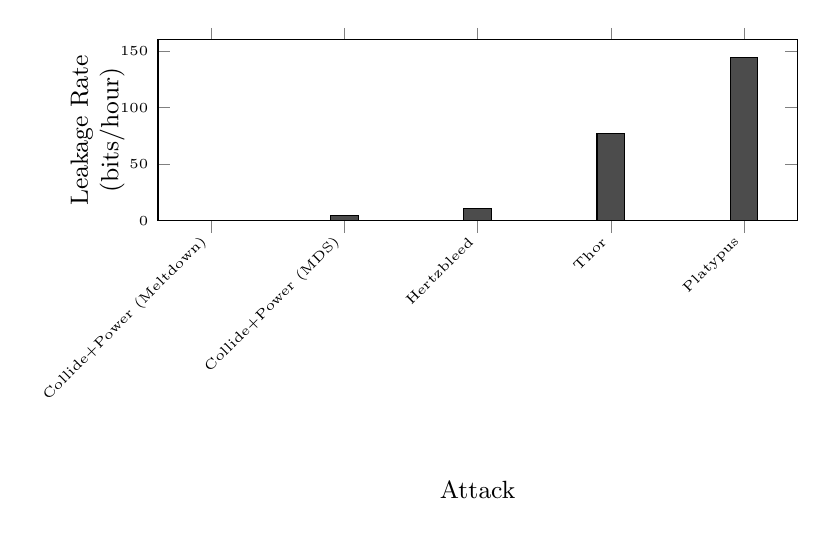
\begin{tikzpicture}
    \begin{axis}[
        ybar,
        symbolic x coords={Collide+Power (Meltdown), Collide+Power (MDS), Hertzbleed, Thor, Platypus},
        xtick=data,
        width=\linewidth*0.8,
        height=\linewidth*0.32,
        xlabel={Attack},
        ylabel={Leakage Rate\\(bits/hour)},
        ymin=0,
        ymax=160,
        x tick label style={
            rotate=45, 
            anchor=east,
            font=\tiny 
        },
        y tick label style={
            font=\tiny 
        },
        bar width=10pt,
        xlabel style={yshift=-0.7cm, font=\small},
        ylabel style={yshift=-0.3cm, align=center, font=\small},
    ]
        \addplot[
        color=black, 
        fill=black!70] coordinates {
            (Collide+Power (Meltdown), 0.136)
            (Collide+Power (MDS), 4.82)
            (Hertzbleed, 10.5)
            (Thor, 76.8)
            (Platypus, 144.7)
        };
    \end{axis}
\end{tikzpicture}
    \caption{\textsc{Thor} leakage rate comparison.}
    \label{fig:thorleakage}
\end{figure}
%
\subsection{Counter-measurement}
\begin{comment}
\textsc{Thor} relies only on precise \textit{timing} measurements. Therefore, it cannot be mitigated by defenses that alter the classification output of NNs, such as adding noise or rounding confidence scores \cite{Fredrikson2015ModelInversion}. 
Trusted Execution Environment (TEE)-based defenses, such as those performing non-linear computations inside the TEE while offloading linear computations to untrusted sources \cite{tramèr2019slalomfastverifiableprivate}, are also inadequate since we confirmed that the value dependencies of Intel AMX timing that \textsc{Thor} relies on are unaffected by TEE environments like Intel SGX. 
AI workloads demand high speed and efficiency, prompting AI libraries to prioritize performance optimizations. As a result, known constant-time programming techniques are often unsuitable as a defense. For example, masking can help protect weights from leaking but introduces extra computational overhead, increasing both power consumption and execution time.
\end{comment}
\textsc{Thor} relies only on precise \textit{timing} measurements. Thus, it cannot be mitigated by defenses that alter NN classification outputs, such as adding noise or rounding confidence scores \cite{Fredrikson2015ModelInversion}. Trusted Execution Environment (TEE)-based defenses, like those performing non-linear computations inside the TEE while offloading linear computations to untrusted sources \cite{tramèr2019slalomfastverifiableprivate}, are also inadequate, as the value dependencies of Intel AMX timing that \textsc{Thor} relies on are unaffected by TEE environments like Intel SGX. AI workloads demand high speed and efficiency, prompting AI libraries to prioritize performance optimizations. As a result, known constant-time programming techniques are often unsuitable as a defense. For example, masking can help protect weights from leaking but introduces extra computational overhead, increasing both power consumption and execution time.

A more effective strategy involves introducing response randomness by delaying execution, which disrupts the timing signals relied upon by \textsc{Thor}. However, this approach adds latency to AI applications. Limiting the query rate of the model 
could also slow these attacks, but at the cost of reducing system responsiveness.
Extending detection mechanisms, 
to identify malicious patterns in power and performance characteristics offers a promising defense against \textsc{Thor}.
Lastly, employing homomorphic encryption 
could provide robust protection but comes with substantial computational overhead and performance costs, making it less practical for high-speed AI applications.


%\subsection{Power \& Performance Overhead}
% In an experiment, we measured the time to execute a single AMX multiplication instruction while varying the intervals between consecutive executions. By adjusting the length of these intervals, we identified five distinct execution times, classifying them into performance states. The shortest execution time with the lowest intervals was labeled as the "Warm State," while the longer execution times with higher intervals were classified as "Cold States." 
One mitigation which can be applied through a micro-code update or a software patch is to keep the AMX unit moderately in the Warm State at all times or at least during Intel SGX execution to protect TEEs computation against \textsc{Thor}.
%
This approach is effective because we observed that timing differences dependent on zero values are only significantly measurable when the Intel AMX is in a Cold State. Warm and Cold States introduced here come from an interesting observation in which 
%In an experiment, 
we measured the time to execute a single AMX multiplication instruction while varying the intervals between consecutive executions. By adjusting the length of these intervals, we identified five distinct execution times, classifying them into performance states. The shortest execution time with the lowest intervals was labeled as the Warm State, while the longer execution times with higher intervals were classified as Cold States.  These performance states are shown in Figure~\ref{fig:Performance_Stages}.
However, this mitigation comes with trade-offs in power management and execution speed, as system power limits could be more easily reached, leading to unnecessary throttling of the AMX unit. We measured the power overhead of such defense for \textsc{Thor} and found that depending on the cold vs. warm stage,  the overhead ranges from 2.59\% to 12.33\%. Although this secure design requires more power consumption, it is faster as it keeps the Intel AMX in the highest performance state at all time; this is in contrary to other secure designs for different microarchitectural attacks which almost always incurred a high performance overhead. 
%\textcolor{red}{Todo  quantitatively calculate the AMX latency in warm state over cold state and add numbers here saying how much faster approx.  }

%Although the secure design requires more power consumption, it could be faster in scenarios such as workloads with infrequent multiplications.
\begin{figure}
    \centering
    \begin{tikzpicture}
        \begin{axis}[
            xmin=100, xmax=1000000000,
            ymin=10, ymax=100000,
            xlabel={Interval Delay (Cycle)},
            ylabel={Multiplication Execution\\Time (Cycle)},
            xmode=log, 
            ymode=log,
            log basis x=10, 
            log basis y=10,
            grid=both,
            major grid style={line width=0pt,draw=white!50},
            minor grid style={line width=0pt,draw=white!20},
            font=\scriptsize,
            ylabel style={yshift=0pt, align=center}, 
            width=\linewidth*1,
            height=\linewidth*0.45,
        ]
            \addplot[darkgray, thick] table {Diagrams/Data/warmup.txt};
        \end{axis}
        
        \draw[->, black, thick] (2.1,0.45) -- (1.1,0.45) node[midway, above] {\scriptsize Warm State};
         \node[gray, thick] at (1.05,1.3) {\scriptsize Cold State 1};
         \node[gray, thick] at (2.8,1.7) {\scriptsize Cold State 2};
         \node[gray, thick] at (4.9,1.85) {\scriptsize Cold State 3};
         \node[gray, thick] at (6.4,2.15) {\scriptsize Cold State 4};
         
    \end{tikzpicture}
    \caption{  Performance States of
TMUL and the Secure Recommended Intel AMX Operational State (Warm).}
    \label{fig:Performance_Stages}
\end{figure}

Thus, future research must prioritize the development of effective mechanisms to mitigate the proposed threat vector introduced by AMX and similar technologies while addressing the secure design's performance and power consumption. 

% \section{Conclusion}
% \section{Conclusion}
In this work, we propose a simple yet effective approach, called SMILE, for graph few-shot learning with fewer tasks. Specifically, we introduce a novel dual-level mixup strategy, including within-task and across-task mixup, for enriching the diversity of nodes within each task and the diversity of tasks. Also, we incorporate the degree-based prior information to learn expressive node embeddings. Theoretically, we prove that SMILE effectively enhances the model's generalization performance. Empirically, we conduct extensive experiments on multiple benchmarks and the results suggest that SMILE significantly outperforms other baselines, including both in-domain and cross-domain few-shot settings.

%\section*{Acknowledgments}
%\begin{acks}
    
\end{acks}

%{\appendix[Proof of the XYZ Equation]
%Hi
%}

%\subsubsection{Conditioned Diffusion Models}

By operating the data in latent space instead of pixel space, conditioned diffusion models have gained promising development \cite{rombach2022latentDiff}. MM-Diffusion \cite{ruan2023mmdi} designed for joint audio and video generation took advantage of coupled denoising autoencoders to generate aligned audio-video pairs from Gaussian noise. Extending the scalability of diffusion models, diffusion Transformers treat all inputs, including time, conditions, and noisy image patches, as tokens, leveraging the Transformer architecture to process these inputs \cite{bao2023ViTDiff}. In DiT \cite{peebles2023DiT}, William et al. emphasized the potential for diffusion models to benefit from Transformer architectures, where conditions were tokenized along with image tokens to achieve in-context conditioning. 

\subsubsection{Diffusion Models in Robotics}

Recently, a probabilistic multimodal action representation was proposed by Cheng Chi et al. \cite{chi2023diffusionpolicy}, where the robot action generation is considered as a conditional diffusion denoising process. Leveraging the diffusion policy, Ze et al. \cite{ze20243d} conditioned the diffusion policy on compact 3D representations and robot poses to generate coherent action sequences. Furthermore, GR-MG combined a progress-guided goal image generation model with a multimodal goal-conditioned policy, enabling the robot to predict actions based on both text instructions and generated goal images \cite{li2025grmg}. BESO used score-based diffusion models to learn goal-conditioned policies from large, uncurated datasets without rewards. Score-based diffusion models progressively add noise to the data and then reverse this process to generate new samples, making them suitable for capturing the multimodal nature of play data \cite{reuss2023md}. RDT-1B employed a scalable Transformer backbone combined with diffusion models to capture the complexity and multimodality of bimanual actions, leveraging diffusion models as a foundation model to effectively represent the multimodality inherent in bimanual manipulation tasks \cite{liu2024rdt-1b}. NoMaD exploited the diffusion model to handle both goal-directed navigation and task-agnostic exploration in unfamiliar environments, using goal masking to condition the policy on an optional goal image, allowing the model to dynamically switch between exploratory and goal-oriented behaviors \cite{sridhar2023nomad}. The aforementioned insights grounded the significant advancements of diffusion models in robotic tasks.

\subsubsection{VLM-based Autonomous Driving}

End-to-end autonomous driving introduces policy learning from sensor data input, resulting in a data-driven motion planning paradigm \cite{chen2024vadv2}. As part of the development of VLMs, they have shown significant promise in unifying multimodal data for specific downstream tasks, notably improving end-to-end autonomous driving systems\cite{ma2024dolphins}. DriveMM can process single images, multiview images, single videos, and multiview videos, and perform tasks such as object detection, motion prediction, and decision making, handling multiple tasks and data types in autonomous driving \cite{huang2024drivemm}. HE-Drive aims to create a human-like driving experience by generating trajectories that are both temporally consistent and comfortable. It integrates a sparse perception module, a diffusion-based motion planner, and a trajectory scorer guided by a Vision Language Model to achieve this goal \cite{wang2024hedrive}. Based on current perspectives, a differentiable end-to-end autonomous driving paradigm that directly leverages the capabilities of VLM and a multimodal action representation should be developed. 








%\section{Background}\label{sec:background}

%\section{Related Work}\label{sec:related_works}
\gls{bp} estimation from \gls{ecg} and \gls{ppg} waveforms has received significant attention due to its potential for continuous, unobtrusive monitoring. Earlier work relied on classical machine learning with handcrafted features, but deep learning methods have since emerged as more robust alternatives. Convolutional or recurrent architectures designed for \gls{ecg}/\gls{ppg} have shown strong performance, including ResUNet with self-attention~\cite{Jamil}, U-Net variants~\cite{Mahmud_2022}, and hybrid \gls{cnn}--\gls{rnn} models~\cite{Paviglianiti2021ACO}. These architectures often outperform traditional feature-engineering approaches, particularly when both \gls{ecg} and \gls{ppg} signals are used~\cite{Paviglianiti2021ACO}.

Nevertheless, many existing methods train solely on \gls{ecg}/\gls{ppg} data, which, while plentiful~\cite{mimiciii,vitaldb,ptb-xl}, often exhibit significant variability in signal quality and patient-specific characteristics. This variability poses challenges for achieving robust generalization across populations. Recent work has explored transfer learning to overcome these issues; for example, Yang \emph{et~al.}~\cite{yang2023cross} studied the transfer of \gls{eeg} knowledge to \gls{ecg} classification tasks, achieving improved performance and reduced training costs. Joshi \emph{et~al.}~\cite{joshi2021deep} also explored the transfer of \gls{eeg} knowledge using a deep knowledge distillation framework to enhance single-lead \gls{ecg}-based sleep staging. However, these studies have largely focused on within-modality or narrow domain adaptations, leaving open the broader question of whether an \gls{eeg}-based foundation model can serve as a versatile starting point for generalized biosignal analysis.

\gls{eeg} has become an attractive candidate for pre-training large models not only because of the availability of large-scale \gls{eeg} repositories~\cite{TUEG} but also due to its rich multi-channel, temporal, and spectral dynamics~\cite{jiang2024large}. While many time-series modalities (for example, voice) also exhibit rich temporal structure, \gls{eeg}, \gls{ecg}, and \gls{ppg} share common physiological origins and similar noise characteristics, which facilitate the transfer of temporal pattern recognition capabilities. In other words, our hypothesis is that the underlying statistical properties and multi-dimensional dynamics in \gls{eeg} make it particularly well-suited for learning robust representations that can be effectively adapted to \gls{ecg}/\gls{ppg} tasks. Our work is the first to validate the feasibility of fine-tuning a transformer-based model initially trained on EEG (CEReBrO~\cite{CEReBrO}) for arterial \gls{bp} estimation using \gls{ecg} and \gls{ppg} data.

Beyond accuracy, real-world deployment of \gls{bp} estimation models calls for efficient inference. Traditional deep networks can be computationally expensive, motivating recent interest in quantization and other compression techniques~\cite{nagel2021whitepaperneuralnetwork}. Few studies have combined large-scale pre-training with post-training quantization for \gls{bp} monitoring. Hence, our method integrates these two aspects: leveraging a potent \gls{eeg}-based foundation model and applying quantization for a compact, high-accuracy cuffless \gls{bp} solution.
\end{spacing}

\begin{spacing}{0.95}
    
%\vspace{-1em}
\bibliographystyle{IEEEtranS}
\bibliography{refs}
\end{spacing}
\vfill
%


% \begin{figure}[!t]
%     \centering
%    \includegraphics[width=\linewidth] {images/AMXarch_new_v1.pdf} 
%     \caption{Intel AMX Architecture Overview}
%     \label{fig:AMX-arch}
% \end{figure}

% \subsection{Intel AMX Architecture and Instructions.}
% Intel AMX is an integrated accelerator introduced with the 4th Gen Intel Xeon Scalable processors, specifically engineered to boost the efficiency of matrix computations. %Figure~\ref{fig:AMX-arch} illustrates the Intel AMX architecture.

% AMX introduces a new set of registers and instructions. The registers in Intel AMX are known as Tiles, a new concept in Intel CPUs that provide a matrix of data registers, as opposed to the traditional vector registers seen in previous SIMD architectures like AVX-512. AMX includes 8 Tile registers, each capable of holding up to 16 rows with 64 bytes per row, amounting to a total of 1 KB per Tile. The number of rows and the number of bytes per row can be adjusted using the LDTILECFG instruction, and this configuration information is stored as metadata in a control register known as TILECFG. Once this configuration is set, AMX instructions such as load, store, and matrix multiplication will operate according to the specified dimensions for each Tile. Intel AMX instructions are synchronized with the Intel Architecture host (IA host) instruction stream, and the Tile loads and stores are coherent with the host memory \cite{Intel_Arc_Ins_Set_Extensions}.

% Tile Matrix Multiply unit (TMUL) serves as the accelerator engine for executing multiplication calculations. When using full-size Tile operands, the latency of the multiplication instruction is 52 cycles, while pipelining allows for a throughput of 16 cycles. Intel AMX supports two data types: BF16 and INT8. Consequently, it can perform 512 multiplications and 512 additions per cycle for BF16 and 1024 multiplications and 1024 additions per cycle for INT8 \cite{IntelOptRefManual}. 

% \begin{comment}
% AMX instructions utilize port 5 as their dedicated execution port. When two hyper-threads are active within a core, they compete for the same resources to execute AMX instructions.
% \end{comment}

\section{Reverse Engineering}
In this section, we share our findings on Intel AMX obtained through reverse engineering. In our investigations, we utilized a server running Red Hat Enterprise Linux release 9.3 (Plow), equipped with Linux kernel version 5.14. The server is powered by two Intel(R) Xeon(R) Gold 5420+ CPUs. 
We did not disable any hardware features or mitigations.

\textbf{Performance States Characterization.} 
In an experiment, we measured how long it takes to execute a single AMX multiplication instruction while varying the intervals between consecutive executions. To simulate the conditions of a typical program, we added non-AMX instructions during these intervals. By changing the length of these intervals, we observed five distinct execution times for the AMX multiplication instruction. We classified these into performance states, with the shortest execution time labeled as the "Warm State." The longer execution times are referred to as "Cold States," specifically Cold State 1 (the second shortest), Cold State 2, Cold State 3, and Cold State 4 (the longest).  Figure \ref{fig:Performance_Stages} visually represents these performance states. 

%\begin{figure}[!hbp]
%\centering\includegraphics[width=0.4\textwidth]{images/sleepstages_new_v2.pdf}
%\caption{Illustration of the Five Distinct Performance States of TMUL.}
%\label{fig:Performance_Stages}
%\end{figure}
%{\color{blue} Change the figure: bias, change the ylabel, and States }

\begin{figure}
    \centering
    \begin{tikzpicture}
        \begin{axis}[
            xmin=100, xmax=1000000000,
            ymin=10, ymax=100000,
            xlabel={Interval Delay (Cycle)},
            ylabel={Multiplication Execution\\Time (Cycle)},
            xmode=log, 
            ymode=log,
            log basis x=10, 
            log basis y=10,
            grid=both,
            major grid style={line width=0pt,draw=white!50},
            minor grid style={line width=0pt,draw=white!20},
            font=\scriptsize,
            ylabel style={yshift=0pt, align=center}, 
            width=\linewidth*1,
            height=\linewidth*0.45,
        ]
            \addplot[darkgray, thick] table {Diagrams/Data/warmup.txt};
        \end{axis}
        
        \draw[->, black, thick] (2.1,0.45) -- (1.1,0.45) node[midway, above] {\scriptsize Warm State};
         \node[gray, thick] at (1.05,1.3) {\scriptsize Cold State 1};
         \node[gray, thick] at (2.8,1.7) {\scriptsize Cold State 2};
         \node[gray, thick] at (4.9,1.85) {\scriptsize Cold State 3};
         \node[gray, thick] at (6.4,2.15) {\scriptsize Cold State 4};
         
    \end{tikzpicture}
    \caption{llustration of the Five Distinct Performance States of
TMUL.}
    \label{fig:Performance_Stages}
\end{figure}

%\begin{spacing}{1}
% \begin{lstlisting}
% for(int i = 0; i < ITERS;i++) {
%   Time = __rdtscp();// Timer
%   for (int k = 0; k < i; k++)// Delay
%      junk = junk + k;
%   cooldown_delay[i] = __rdtscp() - Time; 
%   Time =  __rdtscp()
%   AMX_INSTRUCTION();//e.g_tile_dpbssd(0, 1, 2)
%   execution_time[i] = __rdtscp() - Time; }
% \end{lstlisting}
%\end{spacing}

\textbf{Impact of CPU Frequency on Performance States.} 
In a supplementary experiment, we investigated how changing the CPU frequency, using the "cpufreq" feature, affects the execution time of the previously identified performance states. For this study, we fixed the CPU frequency at various levels and measured the execution times for each performance state without allowing frequency scaling to adjust it dynamically. 

The results are plotted in Figure \ref{fig:Execution_time_vs_Freq}, where each data point represents a specific CPU frequency setting. Execution time was recorded using the `rdtscp` instruction, which operates with a 2 GHz clock frequency reference. We examined frequencies ranging from 800 MHz to 2 GHz in increments of 100 MHz.

Our findings indicate that the execution time of the AMX multiplication instruction in all Cold States is invariant with respect to changes in the current CPU frequency. In contrast, the Warm State execution time is directly proportional to the current CPU frequency.

%\begin{figure}[!hbp]
%\centering\includegraphics[width=0.4\textwidth]{images/Execution_time_vs_Freq.pdf}
%\caption{Execution Time of AMX Multiplication Across Performance States at Varying CPU Frequencies}
%\label{fig:Execution_time_vs_Freq}
%\end{figure}
%{\color{blue} Put Execution\_time\_vs\_Freq figure here}


\begin{figure}[t!]
\centering
\begin{tikzpicture}
    \begin{axis}[
        xlabel={CPU Frequency (MHz)},
        ylabel={Execution time (RDTSCP cycle)},
        legend pos=outer north east,
        font=\scriptsize,
        xlabel style={yshift=0pt},
        ylabel style={yshift=0pt},
        width=\linewidth*0.8,
        height=\linewidth*0.45,
        ymode=log,
        log basis y=10,
        legend style={
                legend columns=1, 
                at={(1.02,0.5)}, 
                anchor=west,   
                font=\tiny,
            },
    ]
    
    \addplot[
        thick,
        mark=diamond,
        line width=1.5pt,
        mark size=3,
        color=darkgray
    ] table {Diagrams/Data/freq4.txt};
    \addlegendentry{Cold State 4};

    \addplot[
        thick,
        mark=x,
        line width=1.5pt,
        mark size=3,
        color=darkgray
    ] table {Diagrams/Data/freq3.txt};
    \addlegendentry{Cold State 3};
 
    \addplot[
        thick,
        line width=1.5pt,
        mark=triangle,
        mark size=2,
        color=darkgray
    ] table {Diagrams/Data/freq2.txt};
    \addlegendentry{Cold State 2};

    \addplot[
        thick,
        mark=star,
        line width=1.5pt,
        mark size=3,
        color=darkgray
    ] table {Diagrams/Data/freq1.txt};
    \addlegendentry{Cold State 1};
   
    \addplot[
        thick,
        line width=1.5pt,
        mark=o,
        mark size=2,
        color=red
    ] table {Diagrams/Data/freq0.txt};
    \addlegendentry{Warm State};



    \end{axis}
\end{tikzpicture}
\caption{Execution Time of AMX Multiplication Across Performance States at Varying CPU Frequencies}
\label{fig:Execution_time_vs_Freq}
\end{figure}

\textbf{Transition Behavior of AMX Frequency to CPU Frequency in Warm State.}
Based on the results presented in Figure \ref{fig:Performance_Stages}, the execution of the TMUL multiplication instruction occurs in Cold State 4 (the longest execution time) when either the operation is performed for the first time or follows a period of inactivity exceeding approximately 20 ms. If subsequent AMX multiplication instructions follow closely, all will operate in the Warm State, which is common in programs with extensive matrix multiplications.

We further examined the execution time in the Warm State immediately after entry, over a fixed duration, across different CPU frequencies. Our observations revealed that the AMX multiplication execution time undergoes a transition period before stabilizing. Closer analysis shows that these variations are related to the AMX's internal frequency adjustments. During this transition period, AMX adjusts its frequency from a lower value towards the current CPU frequency, temporarily using intermediate frequencies.

Figure \ref{fig:Freq_transition} illustrates how the AMX frequency adjusts to align with the CPU frequency. When the CPU frequency is set to 1.2 GHz, the AMX frequency initially ramps up, briefly stabilizes at 1 GHz, and eventually reaches the target frequency of 1.2 GHz. Similarly, when the CPU frequency is fixed at 2 GHz, the AMX frequency transitions through intermediate stages, operating at 1 GHz and 1.3 GHz before stabilizing at 2 GHz.

These findings demonstrate that Intel AMX includes a frequency management unit that controls the operating frequency of the TMUL accelerator. This unit can potentially access or create frequencies that differ from the CPU frequency.

%\begin{figure}[!hbp]
%\centering\includegraphics[width=0.4\textwidth]{images/Freq_transition.pdf}
%\caption{Illustration of AMX Frequency Adjustment During Transition Periods: (a) shows the transition to a 1.2 GHz CPU frequency, with intermediate operation at 1 GHz; (b) demonstrates the adjustment to a 2 GHz CPU frequency, passing through 1 GHz and 1.3 GHz stages.}
%\label{fig:Freq_transition}
%\end{figure}
%{\color{blue} Put Freq\_transition figure here}

\begin{figure}[h!]
\centering
\begin{tikzpicture}
    \begin{axis}[
        xlabel={Number of Instructions},
        ylabel={Execution Time (RDTSCP cycle)},
        legend pos=outer north east,
        font=\scriptsize,
        xlabel style={yshift=5pt},
        ylabel style={yshift=-15pt},
        width=\linewidth*1,
        height=\linewidth*0.45,
        xmin= -0.1,xmax=40000,
        legend style={
                legend columns=-1,
                at={(0.5,1.16)},
                anchor=north, 
                font=\tiny,
                /tikz/column 2/.style={column sep=5pt}, 
            },
    ]
    
    \addplot[
        line width=0.8pt,
        color=black,
    ] table {Diagrams/Data/1400MHz.txt};
    \addlegendentry{1.2 GHz
CPU frequency};


    \addplot[
        line width=0.8pt,
        color=lightgray,
    ] table {Diagrams/Data/2000MHz.txt};
    \addlegendentry{2 GHz
CPU frequency};

    \end{axis}
    
    \node[darkgray, thick] at (2.7,1.57) {\scriptsize 1 GHz};
    \node[darkgray, thick] at (5.7,1.175) {\scriptsize 1.2 GHz};
    \node[darkgray, thick] at (2.5,1.01) {\scriptsize 1.3 GHz};
    \node[darkgray, thick] at (5.5,0.37) {\scriptsize 2 GHz};
\end{tikzpicture}
\caption{Illustration of AMX Frequency Adjustment During Transition Periods: The black graph depicts the transition to a 1.2 GHz CPU frequency, with intermediate operation at 1 GHz; The gray graph demonstrates the adjustment to a 2 GHz CPU frequency, passing through 1 GHz and 1.3 GHz stages.}
\label{fig:Freq_transition}
\end{figure}

\textbf{Impact of Operand Sparsity on TMUL Transition in Warm State.}
In our investigation of the TMUL execution time transition in the Warm State, we discovered an interesting effect involving zero values in the Tile operands during multiplication. By varying the number of zero values in the operands, we observed that increasing the number of zeros accelerates the transition period. This effect is illustrated in Figure \ref{fig:Effect_of_zeros_on_transition}, which presents three graphs depicting operand sparsity levels: 100\% sparsity, 50\% sparsity, and 0\% sparsity. In Figure \ref{fig:Effect_of_zeros_on_transition}, with the CPU frequency fixed at 2 GHz, the results indicate that higher operand sparsity in the Tile operands leads to faster convergence of the TMUL frequency to the CPU frequency.

%\begin{figure}[!hbp]
%\centering\includegraphics[width=0.4\textwidth]{images/Effect_of_zeros_on_transition.pdf}
%\caption{Impact of Operand Sparsity on the Transition Period of TMUL Frequency: The graphs depict the transition behavior with 100\%, 50\%, and 0\% sparsity levels in the Tile operands, showing faster convergence to the CPU frequency with increased sparsity.}
%\label{fig:Effect_of_zeros_on_transition}
%\end{figure}
%{\color{blue} Put Freq\_transition figure here}

\begin{figure}[h!]
\centering
\begin{tikzpicture}
    \begin{axis}[
        xlabel={Number of Instructions},
        ylabel={Execution Time (RDTSCP cycle)},
        legend pos=outer north east,
        font=\scriptsize,
        xlabel style={yshift=5pt},
        ylabel style={yshift=-15pt},
        width=\linewidth*1,
        height=\linewidth*0.48,
        xmin= -0.1,xmax=40000,
        legend style={
                legend columns=-1,
                at={(0.5,1.16)},
                anchor=north, 
                font=\tiny,
                /tikz/column 2/.style={column sep=5pt}, 
            },
    ]
    
    \addplot[
        line width=0.8pt,
        color=black,
    ] table {Diagrams/Data/2000_0Perc.txt};
    \addlegendentry{0\% Sparcity};


    \addplot[
        line width=0.8pt,
        color=lightgray,
    ] table {Diagrams/Data/2000_50Perc.txt};
    \addlegendentry{50\% Sparcity};


    \addplot[
        line width=0.8pt,
        color=gray,
    ] table {Diagrams/Data/2000_100Perc.txt};
    \addlegendentry{100\% Sparcity};

    \end{axis}
    
    \node[darkgray, thick] at (1.2,0.57) {\scriptsize 1.8 GHz};
    \node[darkgray, thick] at (1.9,1.95) {\scriptsize 1 GHz};
    \node[darkgray, thick] at (2,1.23) {\scriptsize 1.3 GHz};
    \node[darkgray, thick] at (5.5,0.4) {\scriptsize 2 GHz};
\end{tikzpicture}
\caption{Impact of Operand Sparsity on the Transition Period of TMUL Frequency: The graphs depict the transition behavior with 100\%, 50\%, and 0\% sparsity levels in the Tile operands, showing faster convergence to the CPU frequency with increased sparsity.}
\label{fig:Effect_of_zeros_on_transition}
\end{figure}

Consequently, the execution time of a program utilizing AMX multiplications is closely associated with the sparsity of its input operands. In Figure \ref{fig:Cumulative_execution_time}, we demonstrate this relationship by executing two test programs with 100 and 1000 AMX multiplications, each with varying Tile operand sparsity levels (0\%, 50\%, and 100\%). To construct the histogram, each scenario was executed 1,000 times. Our results reveal that varying levels of sparsity significantly impact the cumulative execution time of AMX multiplications, with increased sparsity leading to faster program execution.

This discovery uncovers a new value-dependent timing side channel that reveals the sparsity of Tile operands in Intel AMX.

% \begin{figure}[htbp!]
%     \centering
%     \begin{tikzpicture}
%         \begin{axis}[
%             font=\scriptsize,
%             width=\linewidth*0.95,
%             height=\linewidth*0.35,
%             bar width=50,
%             xmin=21800, xmax=24650,
%             xlabel={Execution time (cycle)},
%             ybar,
%             ylabel={Frequency},
%             ylabel style={yshift=-15pt},
%             ymin=0, ymax=0.006,
%             legend style={
%                 at={(0.5,1)}, 
%                 anchor=north, 
%                 legend columns=-1,
%                 font=\scriptsize,
%                 /tikz/column 2/.style={column sep=5pt}, 
%                 fill=none,
%                 draw=none
%             },
%             legend image code/.code={\draw[fill=#1,draw=none] (0cm,-0.1cm) rectangle (0.25cm,0.1cm);},
%             legend entries={100\% sparsity, 50\% sparsity, 0\% sparsity}
%         ]
%             \addplot+[hist={density, bins=50}, fill=lightgray, draw=none] table[y index=0] {Diagrams/Data/100-0.txt};
%             \addplot+[hist={density, bins=50}, fill=black, draw=none] table[y index=0] {Diagrams/Data/100-half.txt};
%             \addplot+[hist={density, bins=50}, fill=gray, draw=none] table[y index=0] {Diagrams/Data/100-1.txt};
%         \end{axis}
%         \node[anchor=south east] at (rel axis cs:-0.05,1) {(a)};
%     \end{tikzpicture}
%     \begin{tikzpicture}
%         \begin{axis}[
%             font=\scriptsize,
%             width=\linewidth*0.95,
%             height=\linewidth*0.35,
%             bar width=50,
%             xmin=35500, xmax=56000,
%             xlabel={Execution time (cycle)},
%             ybar,
%             ylabel={Frequency},
%             ylabel style={yshift=-15pt},
%             ymin=0, ymax=0.0024,
%             legend style={
%                 at={(0.5,1)}, 
%                 anchor=north, 
%                 legend columns=-1,
%                 font=\scriptsize,
%                 /tikz/column 2/.style={column sep=5pt}, 
%                 fill=none,
%                 draw=none
%             },
%             legend image code/.code={\draw[fill=#1,draw=none] (0cm,-0.1cm) rectangle (0.25cm,0.1cm);},
%             legend entries={100\% sparsity, 50\% sparsity, 0\% sparsity}
%         ]
%             \addplot+[hist={density, bins=60}, fill=lightgray, draw=none] table[y index=0] {Diagrams/Data/1000-0.txt};
%             \addplot+[hist={density, bins=60}, fill=black, draw=none] table[y index=0] {Diagrams/Data/1000-half.txt};
%             \addplot+[hist={density, bins=60}, fill=gray, draw=none] table[y index=0] {Diagrams/Data/1000-1.txt};
%         \end{axis}
%         \node[anchor=south east] at (rel axis cs:-0.05,1) {(b)};
%     \end{tikzpicture}
%     \begin{comment}
%     \begin{tikzpicture}
%         \begin{axis}[
%             font=\scriptsize,
%             width=\linewidth*0.95,
%             height=\linewidth*0.5,
%             bar width=50,
%             xmin=170000, xmax=345000,
%             xlabel={Execution time (cycle)},
%             ybar,
%             ylabel={Frequency},
%             ylabel style={yshift=-15pt},
%             ymin=0, ymax=0.00022,
%             legend style={
%                 at={(0.5,1)}, 
%                 anchor=north, 
%                 legend columns=-1,
%                 font=\scriptsize,
%                 /tikz/column 2/.style={column sep=5pt}, 
%                 fill=none,
%                 draw=none
%             },
%             legend image code/.code={\draw[fill=#1,draw=none] (0cm,-0.1cm) rectangle (0.25cm,0.1cm);},
%             legend entries={100\% sparsity, 50\% sparsity, 0\% sparsity}
%         ]
%             \addplot+[hist={density, bins=60}, fill=lightgray, draw=none] table[y index=0] {Diagrams/Data/10000-0.txt};
%             \addplot+[hist={density, bins=60}, fill=black, draw=none] table[y index=0] {Diagrams/Data/10000-half.txt};
%             \addplot+[hist={density, bins=60}, fill=gray, draw=none] table[y index=0] {Diagrams/Data/10000-1.txt};
%         \end{axis}
%         \node[anchor=south east] at (rel axis cs:-0.05,1) {(c)};
%     \end{tikzpicture}
%     \end{comment}
% \begin{comment}
% \caption{Cumulative Execution Time of Programs with Varying Operand Sparsity: The histogram illustrates the effect of operand sparsity on program execution time, highlighting that higher sparsity levels result in quicker execution across different counts of AMX multiplications. Subfigures (a), (b), and (c) represent programs with 100, 1,000, and 10,000 AMX multiplications, respectively.}
% \end{comment}
% \caption{Cumulative Execution Time of Programs with Varying Operand Sparsity: The histogram illustrates the effect of operand sparsity on program execution time, highlighting that higher sparsity levels result in quicker execution across different counts of AMX multiplications. Subfigures (a) and (b) represent programs with 100 and 1,000 AMX multiplications, respectively.}
% \label{fig:Cumulative_execution_time}
% \end{figure}


%\begin{figure}[!htbp]
%\centerline{\includegraphics[width=0.35\textwidth]{images/new_pic.pdf}}
%\caption{Cumulative Execution Time of Programs with Varying Operand Sparsity: The %histogram illustrates the effect of operand sparsity on program execution time, %highlighting that higher sparsity levels result in quicker execution across %different counts of AMX multiplications. Subfigures (a), (b), and (c) represent %programs with 100, 1,000, and 10,000 AMX multiplications, respectively.}
%\label{fig:Cumulative_execution_time}
%\end{figure}

\begin{comment}
\textbf{Operand Patterns Influencing Data-Dependent Timing in AMX Multiplications.}
In this part, we describe specific operand patterns that can accelerate the TMUL frequency transition, thereby reducing cumulative execution time. As previously mentioned, Intel AMX supports both BF16 and Int8 operand types. 

For BF16 operands, we examined both normal values and special values, including zero, subnormal, NaN, and infinity. Consider an element \( x \) in the first Tile operand being multiplied by an element \( y \) in the second Tile operand. Our findings indicate that to expedite the frequency transition, at least one of the operands \( x \) or \( y \) should be zero or subnormal, while the other should be a normal value. In Intel AMX, subnormal values are treated as zeros, meaning that if an input is subnormal, it will be considered as zero. Additionally, if an output element falls into the subnormal range, AMX returns zero for that element. Table \ref{tab:BF16Pattern} lists all possible cases for BF16 operands, highlighting those patterns that facilitate quicker transitions.



\begin{table}[ht]
    \centering
    \resizebox{0.49\textwidth}{!}{%
    \begin{tabular}{|c|c|c|c|}
        \hline
        \backslashbox{Operand 1}{Operand 2} & Normal & Zero/Subnormal & NaN/Inf \\ \hline
        Normal & - & \ding{51} & - \\ \hline
        Zero/Subnormal & \ding{51} & \ding{51} & - \\ \hline
        NaN/Inf & - & - & - \\ \hline
    \end{tabular}
    }
    \caption{BF16 Operand Patterns in Intel AMX: Cases marked with \ding{51} indicate patterns that expedite the TMUL frequency adjustment.}
\label{tab:BF16Pattern}
\end{table}

For Int8 operands, the data-dependent pattern involves zero values in two consecutive Int8 entries within a row. Specifically, this occurs in the \(2k\) and \(2k + 1\) columns of the Tiles, where \(k\) ranges from 0 to \(C/2 - 1\), with \(C\) representing the number of bytes in each row of the Tile. Suppose element \( x(r_1,2i) \) and element \( x(r_1,2i+1) \) in the first Tile are multiplied by element \( y(r_2,2j) \) and element \( y(r_2,2j+1) \) in the second Tile, respectively. Table \ref{tab:Int8Pattern} highlights the combinations of these 4 values that lead to a faster frequency transition.

\begin{table}[ht]
    \centering
    \resizebox{0.47\textwidth}{!}{%
    \begin{tabular}{|c|c|c|c|c|}
        \hline
        \backslashbox{Operand 1}{Operand 2} & [Z, Z] & [Z, N] & [N, Z] & [N, N] \\ \hline
        {[}Z, Z{]} & \ding{51} & \ding{51} & \ding{51} & \ding{51} \\ \hline
        {[}Z, N{]} & \ding{51} & - & \ding{51} & - \\ \hline
        {[}N, Z{]} & \ding{51} & \ding{51} & - & - \\ \hline
        {[}N, N{]} & \ding{51} & - & - & - \\ \hline
    \end{tabular}
    }
    \caption{Int8 Operand Patterns: Entries marked with \ding{51} indicate patterns that accelerate TMUL frequency transition.\newline \small(Z = Zero, N = Non-zero)}
\label{tab:Int8Pattern}
\end{table}

Our results suggest the presence of a zero-skipping mechanism for both BF16 and Int8 operands. The Int8 results indicate that zero-skipping evaluates two bytes concurrently, which is likely due to the simultaneous processing of two Int8 multiplications in a specific pipeline stage within TMUL. Bypassing this pipeline stage necessitates checking both consecutive bytes. We hypothesize that bypassing these Tile element multiplications reduces AMX energy consumption, allowing the frequency management unit to increase TMUL frequency with fewer restrictions. Although the latency and throughput of AMX multiplications are fixed in terms of AMX cycles, they are influenced by operand sparsity when viewed in CPU cycles.

\end{comment}
%\begin{figure}[h]
    \centering
    \includegraphics[width=0.85\linewidth]{SPACE/imgs/figs/fig_attack.pdf}
    \caption{Image corruption operation. We choose 6 representative image corruption operations with different severity (1.0, 3.0, 5.0) and visualized images come from the CIFAR-100 test set.
    }
    \label{fig: attack}
\end{figure}
\end{document}


